%%%Tipo de documento:libro (book),tamaño a4,castellano
\documentclass[a4paper,11pt,twoside,spanish]{book}
% Incluye los parámetros de configuración

%%%%%%%%%%%%%%%%%%%%%%%%%%%%%%%%%%%%%%%%%%%%%%%%%%%%%%%%%%%%%%%%%%%%%
% $Id: preamble.tex, v1.0 misb Exp $
%%%%%%%%%%%%%%%%%%%%%%%%%%%%%%%%%%%%%%%%%%%%%%%%%%%%%%%%%%%%%%%%%%%%%
%%%Para separar correctamente las palabras de multitud de idiomas%%%
\usepackage[spanish,es-noshorthands]{babel}
%Este paquete permite poner acentos directamente. Tipo de codificación
\usepackage[utf8]{inputenc} 

%\usepackage[latin1]{inputenc}
\usepackage[T1]{fontenc}
\usepackage{listings}
\usepackage{multicol}
%\usepackage{ifthen}
\usepackage{pdflscape}%\usepackage{lscape}
\usepackage{tocbibind}
\usepackage{multirow}
\usepackage{float}
\usepackage{eurosym} % to create euro symbol
\usepackage{textcomp} %para poner el +/-

% Incluimos las subsubsections en la tabla de contenidos
\setcounter{tocdepth}{4}
\setcounter{secnumdepth}{3}

% Encabezados quitados en hojas en blanco
\makeatletter
  \def\cleardoublepage{\clearpage\if@twoside \ifodd\c@page\else
  \vspace*{\fill}
    \thispagestyle{empty}
    \newpage
    \if@twocolumn\hbox{}\newpage\fi\fi\fi}
\makeatother


%\usepackage{lscape}
%Better support for graphics. Builds upon the graphics package
\usepackage{graphicx}%[dvips]
%\usepackage[pdftex]{graphicx}
\usepackage{latexsym}
\usepackage{epsfig}
%Paquete para la cabecera de las páginas (nombre, capítulo)
\usepackage{fancyhdr}
\usepackage{color}
%\usepackage{wrapfig}
%\usepackage{subfigure} %\usepackage{subfig}
\usepackage{subcaption}
%\usepackage{epstopdf}
%\usepackage{here}

%%% HIPERVÍNCULOS %%%
%\usepackage[dvipdfm,colorlinks=true,linkcolor=blue]{hyperref}
\usepackage[colorlinks=true,linkcolor=blue]{hyperref}
\hypersetup{ % Cambiar colores 
  colorlinks,
  citecolor=green,
  linkcolor=blue,
  urlcolor= cyan
}

%%% Macros AMS %%%
\usepackage{amsmath}
\usepackage{amsthm}						%%%Macros AMS para teoremas%%%
\usepackage{amsfonts}					%%%Permite usar fuentes AMS%%%
\usepackage{amssymb}					%%%Para usar simbolos AMS%%%

%\usepackage{picins}
\usepackage{boxedminipage}
\usepackage{shadow}
\usepackage{titlesec}
\usepackage{curves}
\usepackage{rotating}
\usepackage{calc}
%\usepackage[below]{placeins}		%%% Situar figuras hasta (incluida) la página donde comienza una nueva sección si en la misma aparece algo de texto de la sección precedente.
\usepackage[section]{placeins}		%%% Figuras dentro de su sección
%\input{Diagrama-Bloques}

%\setcounter{tocdepth}{3}
\spanishdecimal{.}

%--------------------------------------------------------------------------
% Definiciones de estilo de curvas
%--------------------------------------------------------------------------
\definecolor{miazul}{rgb}{0,0,0.9}
\definecolor{mirojo}{rgb}{0.9,0,0}
\def\miestiloa{\curvedashes[1.0mm]{0,0}}
\def\miestilob{\put(0,0){\makebox{}}\color{miazul}\curvedashes[1.0mm]{0}}
\def\miestiloc{\put(0,0){\makebox{}}\color{mirojo}\curvedashes[1.0mm]{0}}
\def\miestilod{\curvedashes[1.0mm]{0.5,0.4}}
%---- Otras posibilidades --------------------------------------------------
%\def\miestilob{\curvedashes[1.0mm]{0.5,0.4}}
%\def\miestiloc{\curvedashes[1.0mm]{0.5,3}}
%---------------------------------------------------------------------------
% Tamaño de las etiquetas en las figuras generadas con el programa de Matlab
%---------------------------------------------------------------------------
\def\tamanoetiquetas{\footnotesize}
\curvewarnfalse   % Evita warning por tramos rectos en una curva
%\curvewarntrue 
%----------------------------------------------------------------------------

\usepackage{anysize} %Soporte para el comando \marginsize
\marginsize{3.5cm}{2.5cm}{2.5cm}{2.5cm}	%Permite manejar los márgenes de forma sencilla
%\input{highlight.sty}
%\usepackage{enumitem}
\usepackage[spanish]{babel}
\usepackage{verbatim} % Para comentario multilínea
\usepackage{listings} % Ignorar símbolos especiales
\usepackage{color} % Colores

%%%%%%%%%%%%%%%%%%%%%%%%%%%%%%%%%%%%%%%%%%%%%%%%%%%%%%%%%%%%%%%%%%%%%%
\title{Plantilla para TFG}
%%%%%%%%%%%%%%%%%%%%%%%%%%%%%%%%%%%%%%%%%%%%%%%%%%%%%%%%%%%%%%%%%%%%%%
%Para evitar que separe las palabras al final de las líneas
\pretolerance=2000
\tolerance=3000
\sloppy
%%%%%%%%%%%%%%%%%%%%%%%%%%%%%%%%%%%%%%%%%%%%%%%%%%%%%%%%%%%%%%%%%%%%%%
%                       TEXTO DEL DOCUMENTO
%%%%%%%%%%%%%%%%%%%%%%%%%%%%%%%%%%%%%%%%%%%%%%%%%%%%%%%%%%%%%%%%%%%%%%
\begin{document}
%Para que aparezca el nombre de tablas y no cuadros.
\renewcommand\tablename{Tabla}
\renewcommand\contentsname{Índice General}
\renewcommand\listfigurename{Índice de Figuras}
\renewcommand\listtablename{Índice de Tablas}
% Formato al enumerar sea: 1.1.1.
\renewcommand\labelenumi{\theenumi.}
\renewcommand{\theenumii}{\arabic{enumii}}
\renewcommand{\labelenumii}{{\theenumi}.\theenumii}
%\renewcommand{\labelenumi}{\arabic{enumi}.}
%\renewcommand{\labelenumii}{\arabic{enumii}.}

% FORMATO DE PÁGINA ______________________________
\addtolength{\headwidth}{\marginparsep}
\addtolength{\footskip}{35pt}
\addtolength{\headwidth}{1.5cm}
\addtolength{\voffset}{-1cm}
\addtolength{\textheight}{1.5cm}
\addtolength{\hoffset}{-1cm}
\addtolength{\oddsidemargin}{1cm}
\addtolength{\evensidemargin}{1cm}
\addtolength{\paperheight}{1cm}

%Numeración romana al inicio del PFC
\frontmatter

%%%%%%%%%%%%%%%%%%%%%%%%%%%%%%%%%%%%%%%%%%%%%%%%%%%%%%%%%%%%%%%%%%%%%%
%                             PORTADA
%%%%%%%%%%%%%%%%%%%%%%%%%%%%%%%%%%%%%%%%%%%%%%%%%%%%%%%%%%%%%%%%%%%%%%
\thispagestyle{empty}
\begin{titlepage}
\begin{center}

%forma de introducir imágenes. el \\[0.5 cm] de final de línea introduce un salto de ese tamaño.
%width=1\textwidth indica el tamaño de la imágen (valores entre 0-1). 
\marginsize{3.5cm}{2.5cm}{2.5cm}{2.5cm} 
\addtolength{\oddsidemargin}{0.8cm}
\vspace{1.3cm}
\begin{figure}[h]
        \centering
\includegraphics[angle=0,width=4cm]{./figuras/uc3m.png}
        \label{fig:escudo}
\end{figure}
\large \textsc{Grado en ingeniería de sistemas audiovisuales} \\ [1 cm]

\large TRABAJO FIN DE GRADO\\[1 cm]

\huge \textsc{Integración de Leapmotion y unity 3D para monitorizar procedimientos de rehabilitación de mano}\\[7 cm]
\end{center}
%flushleft alinea a la izquierda el texto
\begin{flushleft} \Large
\emph{Autor:} Alba Gómez Garrido\\[0.5 cm]
\emph{Tutor:} Mª del Carmen Fernández Panadero  \\
\end{flushleft}

%rellena de blanco el resto de la página para escribir abajo del todo
\vfill

% Bottom of the page
\begin{flushright}
{\large Leganés, Enero 2016}
\end{flushright}

\end{titlepage}
\cleardoublepage
%\newpage
%\thispagestyle{empty} \cleardoublepage

%%%%%%%%%%%%%%%%%%%%%%%%%%%%%%%%%%%%%%%%%%%%%%%%%%%%%%%%%%%%%%%%%%%%%%
%                       TRIBUNAL
%%%%%%%%%%%%%%%%%%%%%%%%%%%%%%%%%%%%%%%%%%%%%%%%%%%%%%%%%%%%%%%%%%%%%%
%\thispagestyle{empty}
%\input{./General/tribunal}
%\newpage
%\thispagestyle{empty} \cleardoublepage

%%%%%%%%%%%%%%%%%%%%%%%%%%%%%%%%%%%%%%%%%%%%%%%%%%%%%%%%%%%%%%%%%%%%%%
%                       AGRADECIMIENTOS
%%%%%%%%%%%%%%%%%%%%%%%%%%%%%%%%%%%%%%%%%%%%%%%%%%%%%%%%%%%%%%%%%%%%%%
\thispagestyle{empty}
\addtolength{\parskip}{10pt}
\chapter{Agradecimientos}
 Alba love
\newpage
%\thispagestyle{empty} \cleardoublepage

%%%%%%%%%%%%%%%%%%%%%%%%%%%%%%%%%%%%%%%%%%%%%%%%%%%%%%%%%%%%%%%%%%%%%%
%                       RESUMEN
%%%%%%%%%%%%%%%%%%%%%%%%%%%%%%%%%%%%%%%%%%%%%%%%%%%%%%%%%%%%%%%%%%%%%%
\cleardoublepage
\thispagestyle{empty} \setlength{\headheight}{-20pt}
\setlength{\topskip}{8pt} \setlength{\textheight}{720pt}
\addtolength{\parskip}{7pt}
%chapter introduce un nuevo capítulo
\chapter{Resumen}

Actualmente las redes sociales están en auge y en continuo crecimiento. Cada vez son más los usuarios que pertenecen a estas comunidades y hacen uso de ellas en su vida cotidiana. Revisar tus redes sociales en determinados momentos del día es un hábito que se ha creado de la necesidad de estar conectados. Este fenómeno ha aumentado con la expansión de los terminales móviles, que hacen posible tener al alcance de la mano su acceso en cualquier momento y lugar. 

En este proyecto se presenta una aplicación centrada en una de las redes sociales de mayor extensión e importancia a día de hoy, Facebook. Se estima que más de un 80\% de la población tiene una cuenta en esta red social. Por eso, gracias a su gran extensión, es una fuente de información de la que se pueden realizar profundos análisis para describir patrones de los perfiles existentes.

La aplicación lleva a cabo un estudio de las páginas de Facebook, ofreciendo un análisis tanto de la información de las propias páginas como un perfilado de los usuarios que siguen dichas páginas. 

El objetivo principal de la aplicación es dar acceso a aquellos individuos, usuarios o no de Facebook, que estén interesados en obtener información de un conjunto de páginas de un mismo sector elegido previamente. 

El estudio se centra en un apartado específico dentro de las páginas de Facebook, llamado \textit{Post to Page}. Esta sección la incluyen muchas empresas, marcas o asociaciones en sus páginas, con el fin de dar libertad de expresión a sus usuarios de una forma directa, facilitando a la entidad establecer una relación más cercana e interactiva con sus seguidores.
 
En este apartado los usuarios suelen expresar su agradecimiento o descontento con algún servicio ofrecido, también escriben mensajes de apoyo ante algún acontecimiento relacionado con la página o meras críticas que resultan ser constructivas para la empresa propietaria de la página en Facebook, ayudándoles a mejorar. Por este motivo, este trabajo de fin de grado se ha centrado en esta sección y ofrece un análisis de datos basado en la atención que reciben los usuarios por parte de las páginas ante sus comentarios y la popularidad de dichos comentarios. Por otra parte, también realiza un perfilado de los usuarios que más comentan en las páginas, con el fin de situarlas en un marco sociocultural.  

\textbf{Palabras clave:} aplicación, crawler, Facebook, red social, minería de datos. 

\chapter{Abstract}

Currently social networks are increasing very quickly. Each day there are more users that belong to those communities and use them regularly. Checking notifications in social networks several times a day has become a habit that generates the need to be connected to the net. This fact has increased with the  expansion of mobile terminals that make the access possible anytime, anywhere.

This work introduces an application focused in one of the biggest and most important social network nowadays, Facebook. It has estimated more than 80\% of population has an account in this social network. Thanks to its big extension, it is a source of information from which can be obtained some  data analysis and user patterns.

The proposed application performs a study of Facebook pages, providing an analysis of both the information of those pages, and a profile of the users following them.

The main objective of the application is to provide access to individuals, whether they are or not Facebook users, who are interested in obtaining a study of a set of pages in the same sector preselect by himself.

The study is focused on a particular section of the Facebook page called \textit{Post to page}. This section is included by many companies, brands or associations in their websites in order to give free expression to their users on a direct way making easy an oncoming with their followers.

In this section, users often express their appreciation or dissatisfaction with any service offered. It is also used to show support to any related event in the page or constructive criticism for the company that owns the page. For this reason, this work is focused in that section, providing data analysis based on the attention to comments users by the pages and the popularity of those. In addition, it is also performed a profile of the users that make more comments in the pages in order to place them in a socio-cultural context.

\textbf{Keywords:} application, crawler, Facebook, social network, data mining.

%%%%%%%%%%%%%%%%%%%%%%%%%%%%%%%%%%%%%%%%%%%%%%%%%%%%%%%%%%%%%%%%%%%%%%
%                       TABLA DE CONTENIDO
%%%%%%%%%%%%%%%%%%%%%%%%%%%%%%%%%%%%%%%%%%%%%%%%%%%%%%%%%%%%%%%%%%%%%%
%Para que cada linea del table of contents este a 0.5mm una de la otra
\pagestyle{empty}
\setlength{\parskip}{0.5mm}
\tableofcontents
\newpage

%%%%%%%%%%%%%%%%%%%%%%%%%%%%%%%%%%%%%%%%%%%%%%%%%%%%%%%%%%%%%%%%%%%%%%
%                       LISTA DE FIGURAS
%%%%%%%%%%%%%%%%%%%%%%%%%%%%%%%%%%%%%%%%%%%%%%%%%%%%%%%%%%%%%%%%%%%%%%
\cleardoublepage
\listoffigures{}
\setlength{\textheight}{685pt}
\thispagestyle{empty}
\cleardoublepage \setlength{\headheight}{12pt}
\thispagestyle{empty}

%%%%%%%%%%%%%%%%%%%%%%%%%%%%%%%%%%%%%%%%%%%%%%%%%%%%%%%%%%%%%%%%%%%%%%
%                       LISTA DE TABLAS
%%%%%%%%%%%%%%%%%%%%%%%%%%%%%%%%%%%%%%%%%%%%%%%%%%%%%%%%%%%%%%%%%%%%%
\cleardoublepage
\listoftables{}
\setlength{\textheight}{685pt}
\thispagestyle{empty}
\cleardoublepage \setlength{\headheight}{12pt}
\thispagestyle{empty}

\cleardoublepage
\chapter{Glosario} 
La lista de los acrónimos utilizados en este proyecto es la siguiente:
\begin{description} 
\item [AMQP] Advanced Message Queuing Protocol 
\item [API] Application Programming Interface
\item [BOE] Boletín Oficial del Estado
\item [CPU] Central Processing Unit (Unidad central de procesamiento)
\item [CRUD] Create, Read, Update and Delete (Crear, Obtener, Actualizar y Borrar)
\item [HTTP] Hypertext Transfer Protocol
\item [IaaS] Infrastructure as a Service
\item [IP] Internet Protocol
\item [MVC] Modelo-Vista-Controlador
\item [Plugin] Complemento 
\item [URL] Uniform Resource Locator
\item [VM] Virtual Machine
\item [XML] eXtensible Markup Language (Lenguaje de marcas extensible)
\item [WWW] World Wide Web
\end{description}

\newpage

\setlength{\textheight}{685pt}
\thispagestyle{empty}
\cleardoublepage \setlength{\headheight}{12pt}
\thispagestyle{empty}



%comenzar con numeración arábica los capítulos del PFC
\mainmatter

%%%%%%%%%%%%%%%%%%%%%%%%%%%%%%%%%%%%%%%%%%%%%%%%%%%%%%%%%%%%%%%%%%%%%%
%                    CAPÍTULOS
%%%%%%%%%%%%%%%%%%%%%%%%%%%%%%%%%%%%%%%%%%%%%%%%%%%%%%%%%%%%%%%%%%%%%%

%Estilo de las páginas: cabeceras con nombre del capitulo, nombre de la sección.
\pagestyle{fancy}
%\pagestyle{headings} Esto me lo pone en cursiva y alineado a la izquierda --> no me gusta
\fancyhf{}
\fancyhead[LE,RO]{\bfseries \thepage}
\fancyhead[LO]{\sffamily\scshape\footnotesize\rightmark}
\fancyhead[RE]{\sffamily\scshape\footnotesize\leftmark}

%Espacio entre párrafos para todo el PFC   
%\setlength{\parskip}{5mm plus 3.5mm minus 1mm}
\addtolength{\parskip}{7pt}
%\usepackage{anysize} %Soporte para el comando \marginsize
%\marginsize{3cm}{3cm}{2.5cm}{2.5cm}    %Permite manejar los márgenes de forma sencilla

% CAPÍTULOS ________________________________________
\chapter{Introducción}

\section{Motivación del proyecto}
La comunicación es uno de los pilares fundamentales de la sociedad en la que vivimos, por ello es una de las vías de conocimiento y transmisión de información. Gracias a la evolución de la tecnología, han evolucionado también los medios de comunicación, abriendo paso a las redes sociales como un medio de comunicación abierto y cercano a la gente.

La acogida de las redes sociales ha sido tan grande que no dejan de crearse nuevas ideas para compartir el día a día. Están en continuo crecimiento, y más aún con la expansión del uso de los \textit{smartphones}, que permiten tenerlas al alcance de la mano en cualquier momento y lugar. Se han convertido en un hábito de la sociedad, como medio de comunicación y como medio de expresión.

Centrándonos en las estadísticas, tal y como muestra \textit{GlobalWebIndex} en su reporte anual de 2015 \cite{2}, hay varias plataformas como Instagram o Pinterest que han crecido exponencialmente en este último año, pero ninguna de ellas  llega al nivel de Facebook. Esta web sigue siendo la red social más popular a nivel mundial, se estima que un 80\% de la población tiene una cuenta en esta red.  
 
Estos hechos suponen una gran motivación en la realización de este proyecto, dado que el estudio realizado se basa en los datos proporcionados por Facebook, esperando obtener un gran volumen de datos fiables dada la gran dimensión de esta plataforma.

Se pretende crear una página web con un registro de usuarios, donde cada usuario pueda adquirir un estudio personalizado. Este estudio se dividirá en dos partes. 

La primera parte realizará un análisis de las páginas de Facebook de su sección \textit{Post to Page}. Este apartado recoge las publicaciones de los usuarios que han visitado la página para poner sus comentarios. Es una parte que no todas las páginas de Facebook tienen activas, por lo que se limitará el estudio a aquellas páginas que la contengan. Los datos se obtendrán consultando a la API de Facebook y se podrán obtener gráficas en relación a las contestaciones a dichos comentarios por parte de la página web, al tiempo de respuesta a los comentarios, y a la popularidad de los comentarios midiendo los "Me gusta" de cada uno.

La segunda parte realizará un estudio de los usuarios que más han publicado en la sección comentada anteriormente, mediante un \textit{crawler}\footnote{Un \textit{crawler} es un robot informático que consulta de manera iterativa cierta información web disponible, con objeto de recopilar datos. Esto será definido más en detalle en la sección \ref{sec:2.3}} que visitará a cada uno de estos usuarios para coger su información pública. Una vez obtenidos los datos, se obtendrán las gráficas en relación a la edad de los usuarios, la localización y la ocupación profesional. 

Con esta aplicación web se podrá definir las características de dichas páginas. Información muy útil de cara al diseño de patrones de empresas o asociaciones, que llevándolo al terreno de los propios integrantes de esta aplicación, podrán conocer los aspectos más destacables de las páginas. 

Destacar que para la realización de la aplicación que hace posible este estudio, no sólo se debe realizar una aplicación web, si no que también hay que llevar a cabo la recopilación de los datos y su posterior procesado, para lo cual se tienen que desarrollar tareas de gran diversidad, que suponen un gran reto para la elaboración de este trabajo fin de grado. 

 
\section{Objetivos del proyecto} \label{sec:1.2}
Con la realización de este proyecto se pretende conseguir una aplicación en la que los usuarios puedan llevar un registro de los análisis realizados a las diferentes páginas de Facebook, de forma que el propio usuario puede conocer las características de un conjunto de  páginas de Facebook que deseen y cuál es el patrón de los usuarios que la siguen. 

Se debe realizar una aplicación web que tenga las siguientes funcionalidades:
\begin{itemize} \itemsep4pt \parskip0pt
\item Registro de nuevos usuarios y función \textit{login/logout} de los usuarios.
\item Opción de búsqueda de un conjunto de páginas de Facebook para su procesado.
\item Procesado general de los datos de la página de Facebook.
\item Procesado en profundidad del perfil de los usuarios.
\item Historial de las búsquedas realizadas. 
\item Presentación de las gráficas de los resultados de cada una de las búsquedas.
\end{itemize}

Para poder realizar estas funcionalidades es necesario el desarrollo de varias partes totalmente distintas, que conformarían el backend de la aplicación. Se enumeran a continuación:
\begin{itemize} \itemsep4pt \parskip0pt
\item Control del registro de usuarios y de cada una de sus búsquedas, almacenandolo en la base de datos.
\item Consultas al API de Facebook para conseguir los datos de las páginas de Facebook.
\item Desarrollo de un \textit{crawler} que recorra cada uno de los usuarios para obtener los datos públicos que proporcionan.
\item Distribución del trabajo en diferentes máquinas virtuales para optimizar el tiempo de procesado de los datos.
\item Procesado de datos, para calcular las estadísticas y representar las gráficas. 
\end{itemize}

\section{Entorno socio-económico}

La idea de este trabajo fin de grado es la creación de una aplicación útil para la sociedad. 
Con esta aplicación se puede beneficiar a las empresas a conocer mejor las características de sus competidores. También se puede utilizar para conocer la reacción de la sociedad ante un suceso importante. 

Por ejemplo, suponiendo el hecho de que hay un corte en las líneas de teléfono móvil durante un día en toda España por un problema técnico. Una de las reacciones de los usuarios sería escribir en las páginas de Facebook para quejarse a sus compañías y esperar una solución acerca de lo sucedido. Con este proyecto se podría ver si realmente la sociedad expresa sus sentimientos en la redes sociales, qué compañía telefónica tiene mayor número de clientes, además con el análisis de los usuarios, se podría conocer el perfil de los usuarios más comunes que se han quejado o han comentado algo al respecto.

Los datos proporcionados por la aplicación, como consecuencia, pueden servir para aplicar tareas de marketing a raíz de los datos obtenidos. Por ejemplo, continuando con el ejemplo de las líneas telefónicas,
identificar qué usuarios se quejan más de los servicios proporcionados con el fin de lanzar campañas de fidelización para los mismos, mejorando su calidad y el impacto de la empresa en cuestión.
 
En definitiva, esta aplicación hace un análisis de una de las redes sociales más importantes hoy en día. Puede llegar a tener un gran valor para las empresas ya que les permite tener \textit{feedback} de sus clientes. Por tanto, este trabajo fin de grado podría llegar a ser un producto comercial. En un contexto socio-económico permitiría la creación de puestos de trabajo.

\section{Estructura del documento}

Tras el primer capítulo de Introducción, el contenido de la presente memoria se completa con 6 capítulos adicionales, los cuales se describen a continuación de forma resumida para facilitar su lectura.

\begin{itemize} \itemsep4pt \parskip0pt
\item \textbf{Glosario}
\item \textbf{Capítulo 1: Introducción} Breve introducción del proyecto en la que se expone la motivación del proyecto, los objetivos que se pretenden lograr, el entorno socio-económico que lo enmarca y la estructura de la memoria.
\item \textbf{Capítulo 2: Estado del arte} Capítulo dedicado al planteamiento del problema, análisis del estado del arte presentando las tecnologías que se han aplicado para el diseño del sistema.
\item \textbf{Capítulo 3: Descripción general del sistema} Visión general del sistema llevado a cabo. Se enumeran los requisitos de las capacidades, funcionalidades y restricciones de las tecnologías aplicadas. Además se plantean las diferentes alternativas y la solución elegida para resolver este proyecto. Por último se describe el entorno de desarrollo utilizado para desenvolver el sistema.
\item \textbf{Capítulo 4: Funcionamiento del sistema} Explicación del funcionamiento del sistema, dividiéndolo en dos grandes bloques: Frontend, que conforma la aplicación web creada, y Backend, que desarrolla toda la parte técnica necesaria para este proyecto.
\item \textbf{Capítulo 5: Ejemplo de utilización de la aplicación} Presentación de un caso práctico para mostrar el funcionamiento de la aplicación.
\item \textbf{Capítulo 6: Planificación del trabajo y presupuesto del proyecto} Planificación seguida para la realización del proyecto y el presupuesto económico necesario para el mismo.
\item \textbf{Capítulo 7: Conclusiones} Conclusiones a las que se han llegado tras la finalización del trabajo y exposición de los posibles trabajos futuros que se podrían implementar para ampliar las funcionalidades de la aplicación.
\item \textbf{Bibliografía}
\end{itemize}

\chapter{Introducción}

\section{Motivación del proyecto}
La comunicación es uno de los pilares fundamentales de la sociedad en la que vivimos, por ello es una de las vías de conocimiento y transmisión de información. Gracias a la evolución de la tecnología, han evolucionado también los medios de comunicación, abriendo paso a las redes sociales como un medio de comunicación abierto y cercano a la gente.

La acogida de las redes sociales ha sido tan grande que no dejan de crearse nuevas ideas para compartir el día a día. Están en continuo crecimiento, y más aún con la expansión del uso de los \textit{smartphones}, que permiten tenerlas al alcance de la mano en cualquier momento y lugar. Se han convertido en un hábito de la sociedad, como medio de comunicación y como medio de expresión.

Centrándonos en las estadísticas, tal y como muestra \textit{GlobalWebIndex} en su reporte anual de 2015 \cite{2}, hay varias plataformas como Instagram o Pinterest que han crecido exponencialmente en este último año, pero ninguna de ellas  llega al nivel de Facebook. Esta web sigue siendo la red social más popular a nivel mundial, se estima que un 80\% de la población tiene una cuenta en esta red.  
 
Estos hechos suponen una gran motivación en la realización de este proyecto, dado que el estudio realizado se basa en los datos proporcionados por Facebook, esperando obtener un gran volumen de datos fiables dada la gran dimensión de esta plataforma.

Se pretende crear una página web con un registro de usuarios, donde cada usuario pueda adquirir un estudio personalizado. Este estudio se dividirá en dos partes. 

La primera parte realizará un análisis de las páginas de Facebook de su sección \textit{Post to Page}. Este apartado recoge las publicaciones de los usuarios que han visitado la página para poner sus comentarios. Es una parte que no todas las páginas de Facebook tienen activas, por lo que se limitará el estudio a aquellas páginas que la contengan. Los datos se obtendrán consultando a la API de Facebook y se podrán obtener gráficas en relación a las contestaciones a dichos comentarios por parte de la página web, al tiempo de respuesta a los comentarios, y a la popularidad de los comentarios midiendo los "Me gusta" de cada uno.

La segunda parte realizará un estudio de los usuarios que más han publicado en la sección comentada anteriormente, mediante un \textit{crawler}\footnote{Un \textit{crawler} es un robot informático que consulta de manera iterativa cierta información web disponible, con objeto de recopilar datos. Esto será definido más en detalle en la sección \ref{sec:2.3}} que visitará a cada uno de estos usuarios para coger su información pública. Una vez obtenidos los datos, se obtendrán las gráficas en relación a la edad de los usuarios, la localización y la ocupación profesional. 

Con esta aplicación web se podrá definir las características de dichas páginas. Información muy útil de cara al diseño de patrones de empresas o asociaciones, que llevándolo al terreno de los propios integrantes de esta aplicación, podrán conocer los aspectos más destacables de las páginas. 

Destacar que para la realización de la aplicación que hace posible este estudio, no sólo se debe realizar una aplicación web, si no que también hay que llevar a cabo la recopilación de los datos y su posterior procesado, para lo cual se tienen que desarrollar tareas de gran diversidad, que suponen un gran reto para la elaboración de este trabajo fin de grado. 

 
\section{Objetivos del proyecto} \label{sec:1.2}
Con la realización de este proyecto se pretende conseguir una aplicación en la que los usuarios puedan llevar un registro de los análisis realizados a las diferentes páginas de Facebook, de forma que el propio usuario puede conocer las características de un conjunto de  páginas de Facebook que deseen y cuál es el patrón de los usuarios que la siguen. 

Se debe realizar una aplicación web que tenga las siguientes funcionalidades:
\begin{itemize} \itemsep4pt \parskip0pt
\item Registro de nuevos usuarios y función \textit{login/logout} de los usuarios.
\item Opción de búsqueda de un conjunto de páginas de Facebook para su procesado.
\item Procesado general de los datos de la página de Facebook.
\item Procesado en profundidad del perfil de los usuarios.
\item Historial de las búsquedas realizadas. 
\item Presentación de las gráficas de los resultados de cada una de las búsquedas.
\end{itemize}

Para poder realizar estas funcionalidades es necesario el desarrollo de varias partes totalmente distintas, que conformarían el backend de la aplicación. Se enumeran a continuación:
\begin{itemize} \itemsep4pt \parskip0pt
\item Control del registro de usuarios y de cada una de sus búsquedas, almacenandolo en la base de datos.
\item Consultas al API de Facebook para conseguir los datos de las páginas de Facebook.
\item Desarrollo de un \textit{crawler} que recorra cada uno de los usuarios para obtener los datos públicos que proporcionan.
\item Distribución del trabajo en diferentes máquinas virtuales para optimizar el tiempo de procesado de los datos.
\item Procesado de datos, para calcular las estadísticas y representar las gráficas. 
\end{itemize}

\section{Entorno socio-económico}

La idea de este trabajo fin de grado es la creación de una aplicación útil para la sociedad. 
Con esta aplicación se puede beneficiar a las empresas a conocer mejor las características de sus competidores. También se puede utilizar para conocer la reacción de la sociedad ante un suceso importante. 

Por ejemplo, suponiendo el hecho de que hay un corte en las líneas de teléfono móvil durante un día en toda España por un problema técnico. Una de las reacciones de los usuarios sería escribir en las páginas de Facebook para quejarse a sus compañías y esperar una solución acerca de lo sucedido. Con este proyecto se podría ver si realmente la sociedad expresa sus sentimientos en la redes sociales, qué compañía telefónica tiene mayor número de clientes, además con el análisis de los usuarios, se podría conocer el perfil de los usuarios más comunes que se han quejado o han comentado algo al respecto.

Los datos proporcionados por la aplicación, como consecuencia, pueden servir para aplicar tareas de marketing a raíz de los datos obtenidos. Por ejemplo, continuando con el ejemplo de las líneas telefónicas,
identificar qué usuarios se quejan más de los servicios proporcionados con el fin de lanzar campañas de fidelización para los mismos, mejorando su calidad y el impacto de la empresa en cuestión.
 
En definitiva, esta aplicación hace un análisis de una de las redes sociales más importantes hoy en día. Puede llegar a tener un gran valor para las empresas ya que les permite tener \textit{feedback} de sus clientes. Por tanto, este trabajo fin de grado podría llegar a ser un producto comercial. En un contexto socio-económico permitiría la creación de puestos de trabajo.

\section{Estructura del documento}

Tras el primer capítulo de Introducción, el contenido de la presente memoria se completa con 6 capítulos adicionales, los cuales se describen a continuación de forma resumida para facilitar su lectura.

\begin{itemize} \itemsep4pt \parskip0pt
\item \textbf{Glosario}
\item \textbf{Capítulo 1: Introducción} Breve introducción del proyecto en la que se expone la motivación del proyecto, los objetivos que se pretenden lograr, el entorno socio-económico que lo enmarca y la estructura de la memoria.
\item \textbf{Capítulo 2: Estado del arte} Capítulo dedicado al planteamiento del problema, análisis del estado del arte presentando las tecnologías que se han aplicado para el diseño del sistema.
\item \textbf{Capítulo 3: Descripción general del sistema} Visión general del sistema llevado a cabo. Se enumeran los requisitos de las capacidades, funcionalidades y restricciones de las tecnologías aplicadas. Además se plantean las diferentes alternativas y la solución elegida para resolver este proyecto. Por último se describe el entorno de desarrollo utilizado para desenvolver el sistema.
\item \textbf{Capítulo 4: Funcionamiento del sistema} Explicación del funcionamiento del sistema, dividiéndolo en dos grandes bloques: Frontend, que conforma la aplicación web creada, y Backend, que desarrolla toda la parte técnica necesaria para este proyecto.
\item \textbf{Capítulo 5: Ejemplo de utilización de la aplicación} Presentación de un caso práctico para mostrar el funcionamiento de la aplicación.
\item \textbf{Capítulo 6: Planificación del trabajo y presupuesto del proyecto} Planificación seguida para la realización del proyecto y el presupuesto económico necesario para el mismo.
\item \textbf{Capítulo 7: Conclusiones} Conclusiones a las que se han llegado tras la finalización del trabajo y exposición de los posibles trabajos futuros que se podrían implementar para ampliar las funcionalidades de la aplicación.
\item \textbf{Bibliografía}
\end{itemize}

%%%%%%%%%%%%%%%%%%%%%%%%%%%%%%%%%%%%%%%%%%%%%%%%%%%%%%%%%%%%%%%%%%%%%
%                       DESCRIPCIÓN GENERAL
%%%%%%%%%%%%%%%%%%%%%%%%%%%%%%%%%%%%%%%%%%%%%%%%%%%%%%%%%%%%%%%%%%%%%
\chapter{Descripción general del sistema}
En este capítulo se van a describir las características principales de la aplicación, las herramientas utilizadas para su desarrollo y los requisitos necesarios para poder llevar a cabo las funcionalidades descritas en la sección \ref{sec:1.2}.

\section{Presentación}
El objetivo principal de este trabajo fin de grado es la creación de una aplicación web que sea capaz de analizar un conjunto de páginas de \textit{Facebook} de manera automática. 

La figura (\ref{fig:general}) muestra un esquema general de la aplicación:

\begin{figure}[H]
\centering
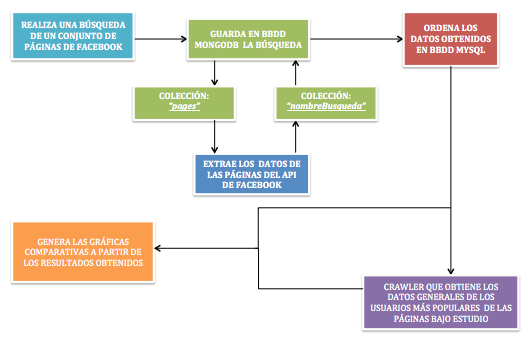
\includegraphics[width=5in]{figuras/esquemaGeneral.png}
\caption{Esquema general del proyecto} \label{fig:general}
\end{figure}

Siguiendo este esquema, primero el usuario debe indicar el nombre del estudio que va a realizar, el nombre de las páginas y el periodo de tiempo que lo engloban, y una dirección de correo electrónico para enviarle una notificación cuando la recopilación de datos haya finalizado. También debe seleccionar si desea que el estudio se haga sólo de las páginas de \textit{Facebook} o también de los usuarios más comunes. Una vez realizada la petición por parte del usuario, la aplicación web internamente se encarga de la recopilación de datos.
 
Para la recolección de los datos, primero guarda la búsqueda del usuario en una base de datos en MongoDB, en una colección llamada "pages". 

Acto seguido, realiza una petición al API de \textit{Facebook}, solicitando los datos contenidos en la sección \textit{Post to Page} de cada una de las páginas dentro del periodo de tiempo solicitado por el usuario. Esta petición devuelve los datos que son automáticamente guardados en la base de datos de MongoDB, en una colección creada con el mismo nombre que ha indicado el usuario para su estudio. 

A continuación, se procesan los datos en una base de datos relacional, MySQL, que permite estructurar los datos obtenidos de la Plataforma de \textit{Facebook}, guardando sólo aquellos campos que nos interesan y ordenándolos para facilitar su posterior procesado.

Una vez finalizado este paso, si el usuario ha seleccionado la opción del estudio de usuarios, por un lado se procede a la extracción de sus datos y por otro lado, se manda un primer informe al usuario de la aplicación con las gráficas de los datos obtenidos de \textit{Facebook}. Proceso que se repite cuando la recopilación de datos de los usuarios haya finalizado.    

Se trata de una aplicación clara y sencilla en la que los usuarios puedan comparar el análisis de diferentes páginas de \textit{Facebook} dentro de su sesión, llevando un historial que almacena todas las peticiones realizadas. 

\section{Requisitos necesarios}
En esta sección se van a definir los requisitos necesarios para el desarrollo técnico de la aplicación propuesta. También se definen los requisitos y restricciones de las tecnologías utilizadas.
\subsection{Requisitos de la aplicación}
A continuación se enumeran todos los requisitos y necesidades que se considera que debe realizar la herramienta a desarrollar, que afectan sólo al portal web. 
\begin{enumerate} \itemsep4pt \parskip0pt
\item \textbf{Accesible desde distintos navegadores}

Los navegadores más comunes, "Mozilla Firefox", "Google Chrome", "Safari", "Internet Explorer", podrán utilizar la aplicación.
\item \textbf{Idioma} \\
El idioma de la aplicación será el español.
\item \textbf{Registro de usuarios} \\
El usuario deberá registrarse previamente para usar la  aplicación.
\item \textbf{Inicio de sesión} \\ 
El usuario deberá haber iniciado sesión con una cuenta registrada para acceder a la aplicación.
\item \textbf{Nueva búsqueda: Nombre estudio} \\
El usuario deberá indicar el nombre del estudio que quiere realizar.
\item \textbf{Nueva búsqueda: Nombre páginas de Facebook} \\
El usuario deberá indicar el nombre de las páginas que quiere analizar, asegurándose primero de que estas páginas contengan la sección \textit{Post to Page}.
\item \textbf{Nueva búsqueda: Periodo del estudio} \\
El usuario deberá indicar la fecha de inicio del estudio, es decir, desde cuando quiere que sea el primer comentario recogido en el estudio hasta la fecha actual. 
\item \textbf{Nueva búsqueda: Correo Electrónico} \\
El usuario deberá indicar una cuenta de correo electrónico donde se le enviará una notificación cuando la recopilación de datos haya acabado. 
\item \textbf{Nueva búsqueda: Opción informe de las páginas}\\
Si el usuario selecciona esta opción se procederá a la recolección de datos de las páginas indicadas obteniéndolos del API de \textit{Facebook}, y se representarán las gráficas comparativas con los resultados obtenidos.
\item \textbf{Nueva búsqueda: Opción informe de los usuarios} \\
Si el usuario selecciona esta opción se procederá a la extracción de datos de los usuarios que más comentan en dicha sección de \textit{Facebook}. Se obtendrán los datos de los usuarios de su fecha y lugar de nacimiento, edad y ocupación profesional mediante un \textit{crawler}.
\item \textbf{Historial de búsquedas} \\
Los usuarios tendrán acceso a todas las búsquedas que hayan realizado en la aplicación, se mostrarán en una tabla.
\item \textbf{Ver análisis} \\
Los usuarios dentro del historial de búsqueda podrán acceder a ver el análisis de cada uno de los estudios, se representarán las gráficas más representativas de los datos obtenidos. 
\item \textbf{Cerrar sesión} \\
Los usuarios podrán cerrar sesión cuando quieran, para mantener seguros sus estudios. 
\item \textbf{Web responsiva} \\
La interfaz web deberá adaptarse a cualquier tamaño de pantalla.
\item \textbf{Lenguajes de programación} \\
Los lenguajes de programación para el desarrollo de la aplicación serán: Java, JSP, HTML, CSS, XML, JavaScript y jQuery.
\end{enumerate}

\subsection{Requisitos de Facebook}
En este epígrafe se describirán los requisitos que Facebook impone para el correcto desarrollo de la aplicación que se pretende seguir. 
\begin{enumerate} \itemsep4pt \parskip0pt
\item \textbf{Soporte HTTP}\\
El servidor donde se aloje debe soportar peticiones HTTP Get y Post.
\item \textbf{Cuenta en Facebook} \\
Para poder acceder a \textit{Facebook}, se debe tener creada una cuenta en dicha red social.
\item \textbf{Cuenta de desarrollador} \\
Para poder acceder a la Plataforma de \textit{Facebook} y a su API, se debe crear crear una cuenta de desarrollador, esto es, aceptar los permisos y condiciones que indican desde una cuenta de \textit{Facebook} de usuario.
\item \textbf{Crear una aplicación en Facebook}\\
Para poder hacer peticiones a la API se necesita crear una aplicación dentro de la Plataforma, que proporcionará las credenciales necesarias para dichas peticiones.
\end{enumerate}

\subsection{Requisitos del crawler}
En este apartado se definirán las condiciones necesarias para poder ejecutar el \textit{crawler} en el entorno adecuado.
\begin{enumerate} \itemsep4pt \parskip0pt
\item \textbf{Máquinas virtuales con interfaz gráfica}\\
Para poder simular la acción de un usuario normal de \textit{Facebook} que recopile los datos de los usuarios a los que visita, se necesitará acceso a máquinas virtuales con entorno gráfico, donde se ejecutará el \textit{crawler} que lanzará instancias de un navegador para simular esta acción.
\item \textbf{Java} \\
El lenguaje de programación será Java, por lo que habrá que instalar el entorno de Java en la máquinas que se vaya a ejecutar. 
\item  \textbf{Número de identificación de los usuarios de \textit{Facebook}} \\
Se necesitarán los \textit{ids} de aquellos usuarios que se vayan a analizar mediante el \textit{crawler}.
\item  \textbf{Distribución del crawler} \\
Se utilizará un software de distribución de paquetes, RabbitMQ, para optimizar el tiempo de ejecución del \textit{crawler}. Desde la aplicación se mandará a cada máquina virtual, mediante este mecanismo, el trabajo que debe realizar cada una.
\end{enumerate}

\subsection{Requisitos de desarrollo}
Por último se expondrán los requisitos necesarios para la elaboración de este proyecto.
\begin{enumerate} \itemsep4pt \parskip0pt
\item \textbf{Espacio para el trabajo} \\
Se dispondrá de una espacio lo suficientemente amplio para poder albergar el equipo de trabajo.
\item \textbf{Ordenador} \\
Se necesitará un ordenador para el desarrollo del trabajo fin de grado.
\item \textbf{Conexión a internet} \\
Se necesitará conexión a Internet para la completa realización del proyecto.
\item \textbf{Servidor} \\
Se necesitará un servidor donde alojar las máquinas virtuales.
\item \textbf{Servidor web y bases de datos}
Se requerirá un servidor web donde alojar la aplicación web y deberá soportar el almacenamiento de los datos en bases de datos. 
\end{enumerate}

\section{Alternativas de implementación del sistema}
\subsection{Alternativas del lenguaje}
Una vez planteadas las tecnologías a desarrollar y los requisitos necesarios, se tuvieron en cuenta las posibilidades de los lenguajes de programación para aplicar al proyecto. 
Para el desarrollo de una aplicación web se utilizan tres lenguajes indispensables, HTML, CSS y JavaScript, para el diseño de las vistas. Sin embargo, para integrar la aplicación con la API de \textit{Facebook} y para el manejo de las bases de datos se pueden utilizar varios lenguajes como Java, Python o Ruby, que disponen de librerías para facilitar el acceso a estas tecnologías.
También se analizaron las posibilidades para el desarrollo del "\textit{crawler}" basado en la herramienta de pruebas de Selenium-WebDriver. Esta herramienta está completamente implementada y soportada en Java, Ruby, Python y C\#. 
\subsection{Evaluación de las alternativas de lenguaje y elección de la solución}
Como las alternativas disponibles para el desarrollo de las tecnologías que conforman el núcleo de este trabajo fin de grado se podían desarrollar indistintamente en varios lenguajes, finalmente se decidió el lenguaje de programación Java. 
Una de las ventajas de decidir Java es que es programación orientada a objetos, simplifica mucho el código y el desarrollo definiendo los objetos necesarios y reutilizándolos. Otra de las ventajas es que es multiplataforma, funciona en todos los entornos disponibles. Es completamente gratis y no depende de ninguna licencia. 
\subsection{Alternativas de las bases de datos}
A la hora de decidir el tipo de bases de datos a utilizar, se tuvo que tener en cuenta el motor principal de este trabajo fin de grado, que es la API de Facebook. Las consultas que se realizan a Facebook, la API las devuelve en formato JSON, y con una estructura variable, dependiendo de los datos que proporciona cada página. 
Por este motivo, se estudió la posibilidad de usar una base de datos NoSQL, que permitiera almacenar los datos sin un esquema predefinido.
Existen varias posibilidades de bases de datos no relacionales como son Cassandra, Redis, MongoDB y CouchDB.
Pero por otro lado, de cara al análisis de datos que esta aplicación recogerá, se consideró que sería conveniente tener una base de datos organizada, almacenando los datos de interés para el análisis. Varias de las alternativas planteadas fueron: MySQL, Access, PostgreesSQL, Microsoft SQL.  
\subsection{Evaluación de las alternativas de bases de datos y elección de la solución}
Dentro de los tipos de bases de datos relacionales, se eligió una base de datos en MySQL, porque aunque todos los tipos cumplían los requisitos necesarios para la implementación de este trabajo fin de grado, MySQL se caracteriza por la rapidez de acceso a la información, punto interesante de cara a cargar los datos en una página web. Además el volumen de datos almacenado no será muy grande, otro aspecto por los que se eligió MySQL. 

En cuanto a las opciones de bases de datos no relacionales la elección fue más fácil. Se eligió MongoDB porque se pueden almacenar los datos BSON directamente, que es una evolución de JSON, esto facilita las peticiones realizadas a la API de Facebook, pudiendo almacenar el JSON que devuelve, sin tener que comprobar si están todos los campos, o si añade uno nuevo. Además de que es un bastante rápido a la hora de ejecutar las operaciones.
\subsection{Alternativas del diseño web}
El Frontend que conformará la interfaz de usuario, para esta parte se utilizará HTML, CSS para definir los estilos y JavaScript y jQuery para añadir efectos y funcionalidades a la página. 
Por otro lado, para el Backend, se estudiaron las distintas posibilidades para generar las páginas de forma dinámica. En esta parte, hubo que decidir el lenguaje de programación adecuado. Estos lenguajes, en el lado del servidor, buscarán la información en una base de datos para mostrarla en la interfaz. Existen varias posibilidades como son PHP, Python, Ruby, ASP.NET o Java.
\subsection{Evaluación de las alternativas de diseño web y elección de la solución} \label{sec:3.3.6}
El diseño web fue el último punto de este proyecto que se decidió, debido a que la importancia del trabajo era recopilar los datos de Facebook. Por tanto, una vez definido como lenguaje de programación Java, y teniendo tanto el \textit{crawler} como el programa que accede a la API de Facebook en Java, se estudiaron las opciones disponibles de hacer una aplicación que implementara sin ningún tipo de problema los scripts comentados. Por esta misma razón se decidió realizar la aplicación web en la plataforma Java, utilizando Spring, que es un framework para el desarrollo de aplicaciones para la plataforma Java. Concretamente. Spring-MVC, módulo que implementa la arquitectura de Modelo-Vista-Controlador.

Destacar que el diseño de la aplicación se ha llevado acabo utilizando dos plantillas de Bootstrap. Bootstrap es un \textit{framework} CSS, que permite dar forma a un sitio web utilizando librerías CSS ya definidas. Una de las plantillas se ha utilizado para los formularios de Inicio de Sesión y de Registro, esta plantilla se llama  "Sign In Bootstrap Template" y se puede encontrar en el enlace \cite{login}. Estas plantillas se han modificado acorde a la estética de la aplicación. La otra plantilla se ha utilizado para el formulario de una nueva búsqueda, y ha definido el estilo que sigue la aplicación, se llama "Multi Step Registration Form" y se puede encontrar en el enlace \cite{step}. 
\section{Entorno de desarrollo utilizado}

\subsection{Eclipse IDE for Java EE Developers}

El programa utilizado para implementar el código de la aplicación es Eclipse \cite{3}. Es un programa informático compuesto por un conjunto de herramientas de programación de código abierto multiplataforma. 

Para desarrollar este proyecto se han utilizado dos plugins disponibles en el entorno de desarrollo. Un plugin es un complemento que se instala en el entorno de desarrollo, facilitan y agilizan el desarrollo.

Un plugin utilizado es el de Maven \cite{3}, Maven es una herramienta de gestión de proyectos. Se basa en un fichero central pom.xml, donde se definen todas las dependencias necesarias para el proyecto. Maven maneja las dependencias del proyecto, se las descarga y las añade al \textit{classpath}. Otro puglin necesario es el de Spring, Spring es un \textit{framework} para el desarrollo de aplicaciones de código abierto para la plataforma Java. En este proyecto se ha utilizado la versión 3 del \textit{framework}, que permite definir una arquitectura de software Modelo-Vista-Controlador. Esta arquitectura define por un lado los componentes para la representación de la información, y por otro lado para la interacción del usuario.

En las figuras (\ref{fig:esqEclipseB}) y (\ref{fig:esqEclipseF}) se presenta el esquema seguido para el desarrollo del trabajo de fin de grado en Eclipse. 

\begin{figure}[H]
\centering
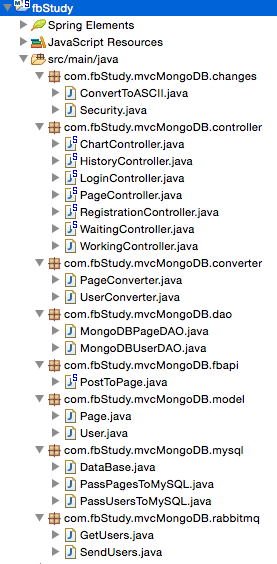
\includegraphics[width=3.2in]{figuras/esquemaBackend.png}
\caption{Esquema TFG en Eclipse. Parte 1} \label{fig:esqEclipseB}
\end{figure}

\begin{figure}[H]
\centering
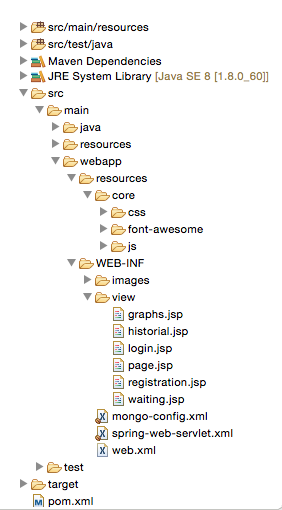
\includegraphics[width=3.5in]{figuras/esquemaFrontend.png}
\caption{Esquema TFG en Eclipse. Parte 2} \label{fig:esqEclipseF}
\end{figure}

Como se puede observar en los esquemas anteriormente mostrados, dentro de la carpeta "src/main/java" se ha definido un paquete para cada una de las funcionalidades implementadas, además de las propias necesarias para el correcto funcionamiento de la aplicaciones web siguiendo la estructura MVC. 

Por otro lado en la carpeta "webapp" se definen todas las vistas necesarias para la aplicación web, además de los estilos y plantillas utilizadas, y la configuración del servidor web, que se describe en el siguiente apartado \ref{sec:1.2}.

A continuación en las tablas (\ref{tab:clases1}) y (\ref{tab:clases2}), se detalla la funcionalidad de las clases mostradas en los esquemas anteriores:
\begin{table}[H]
	\centering
	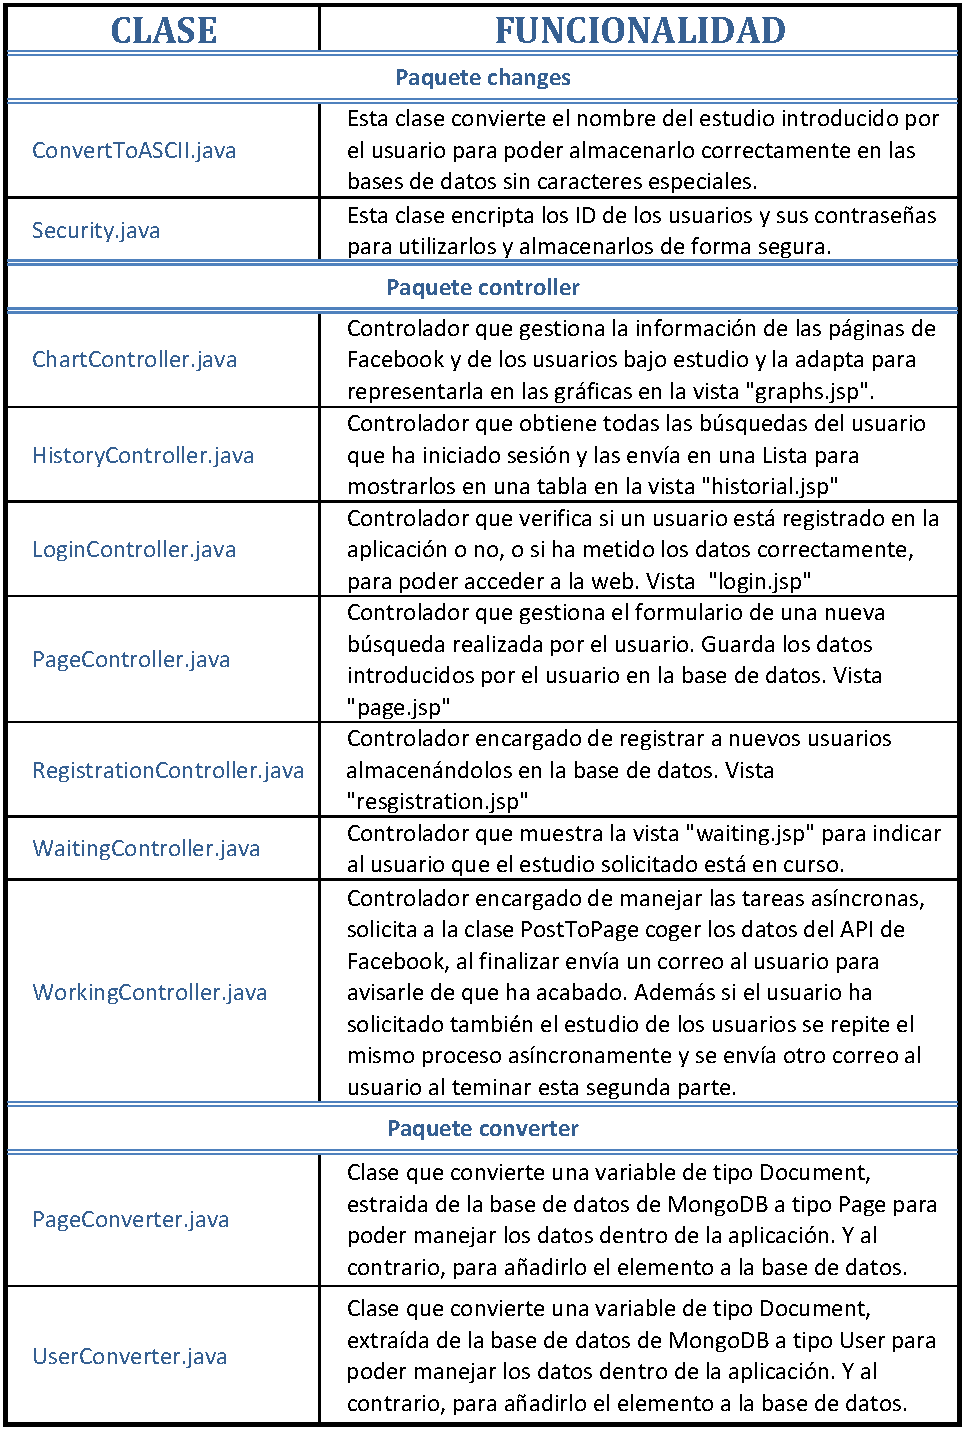
\includegraphics[width=5.2in]{PDF/Clasesjava1.pdf}
	\caption{Clases de java definidas en el proyecto. Parte 1}
	\label{tab:clases1}
\end{table}
\begin{table}[H]
	\centering
	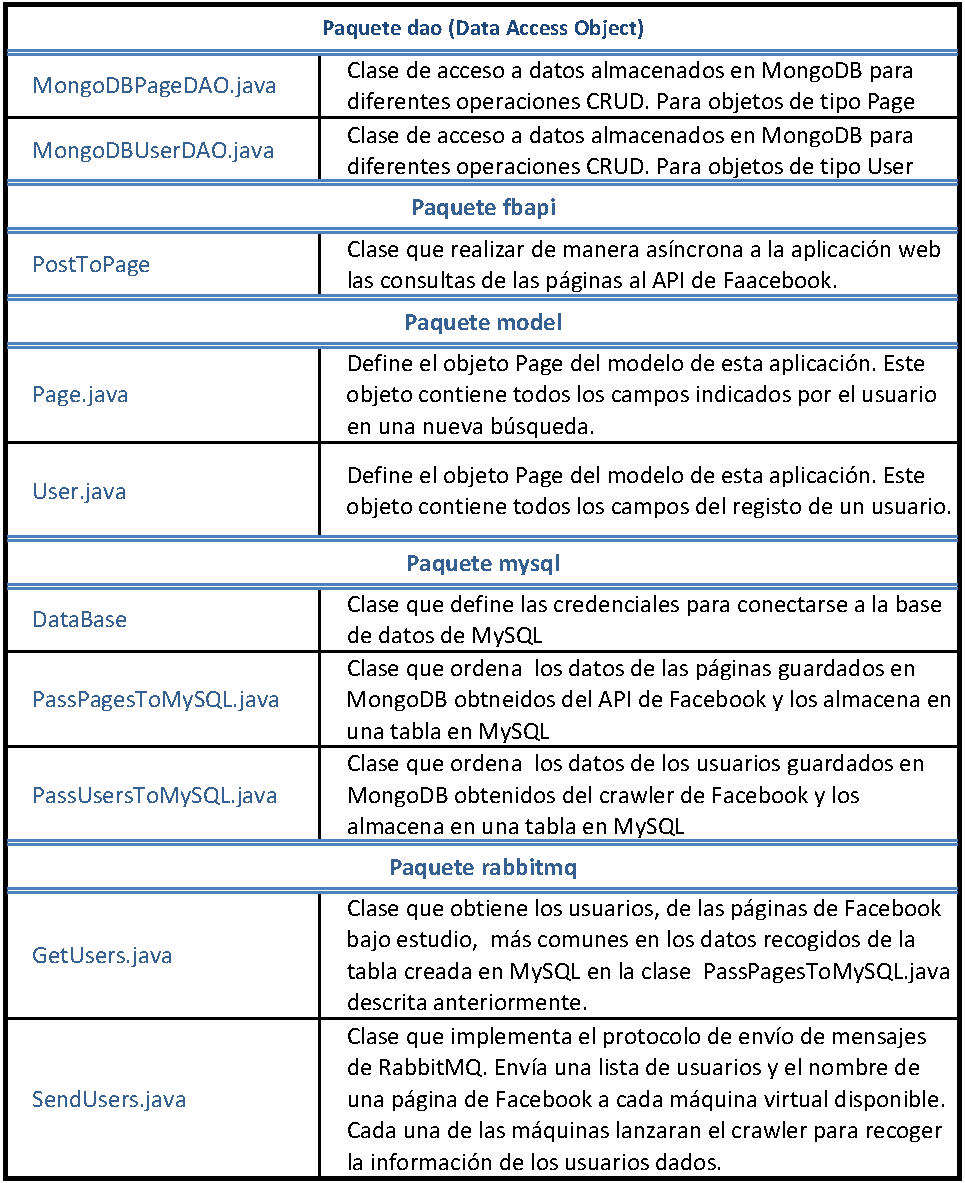
\includegraphics[width=5in]{PDF/Clasesjava2.pdf}
	\caption{Clases de java definidas en el proyecto. Parte 2}
	\label{tab:clases2}
\end{table}
\subsection{Servidor web Jetty} \label{sec:1.2}
\begin{figure}[H]
\centering

\includegraphics[width=2in]{figuras/logoJetty.jpg}
\caption{Logo Servidor Web Jetty} \label{fig:logoJetty}
\end{figure}

Jetty es un Servidor Web y Contenedor de \textit{Servlet}s preparado para ser embebido en las aplicaciones. Es un proyecto de software libre y está completamente basado en Java. 
Los motivos por los que se ha usado este servidor en concreto son los siguientes: \\
\begin{itemize} \itemsep4pt \parskip0pt
\item Es ligero y eficiente
\item Está alojado en Eclipse
\item Basado en Java
\item Soporta peticiones HTTP POST y GET
\item Procesa peticiones asíncronas, capaz de manejar el mecanismo de consulta larga
\end{itemize}

Además de cumplir todos los requisitos necesarios para este proyecto, otro de los motivos por los que se ha utilizado es por la simplicidad de su configuración, basta con definirlo en un fichero XML o en una clase java e incluir sus dependencias en el fichero pom.xml. Con estos dos pasos, la aplicación se ejecuta directamente desde este servidor web.

\begin{figure}[H]
\centering
{
\setlength{\fboxsep}{0pt}
\setlength{\fboxrule}{1pt}
\fbox{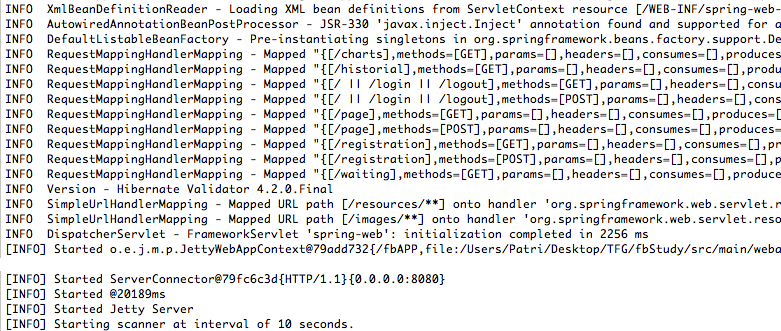
\includegraphics[width=6in]{figuras/ejemplolog.png}}
}
\caption{Registro del servidor web Jetty} \label{fig:log}
\end{figure}


%%%%%%%%%%%%%%%%%%%%%%%%%%%%%%%%%%%%%%%%%%%%%%%%%%%%%%%%%%%%%%%%%%%%%
%                       DESCRIPCIÓN DETALLADA
%%%%%%%%%%%%%%%%%%%%%%%%%%%%%%%%%%%%%%%%%%%%%%%%%%%%%%%%%%%%%%%%%%%%%
\chapter{Funcionamiento del sistema}

Para explicar en profundidad el funcionamiento de la aplicación web, se va a describir dividiéndolo en dos grandes grandes bloques, por un lado la parte del cliente, lo que el usuario ve, denominado frontend, y por otro lado la parte del servidor, cómo está distribuido el sistema para poder realizar todas las funcionalidades, denominado backend.

\section{Frontend}
En el frontend se define la interfaz de usuario. Como ya se ha descrito en la sección (\ref{sec:3.3.6}), la aplicación web está basada en Spring MVC. Se trata de un Modelo-Vista-Controlador. 

En esta sección se va a definir la Vista, que depende directamente del Modelo que se ha definido para que el usuario pueda interactuar con la aplicación. Además de indicar qué acciones realiza el Controlador para el correcto funcionamiento de cada una de las vistas detallas.

En el Modelo de esta aplicación se han diseñado dos objetos: 
\begin{itemize} \itemsep4pt \parskip0pt
\item Modelo User: define todos los campos de información relacionados con el usuario.  
\item Modelo Page: define todos los campos de información relacionados con la búsqueda de páginas.
\end{itemize}
Una vez definido el Modelo, la Vista ya puede interactuar con ellos mediante el Controlador que los maneja. 
Un Controlador responde a eventos, acciones del usuario, e invoca peticiones al Modelo cuando se hace alguna solicitud sobre la información. Cada Controlador se encarga de una vista, definidos en la tabla (\ref{tab:clases1}). 

Para facilitar el desenlace de este apartado en la figura (\ref{fig:web}) representa un diagrama del funcionamiento de la web básico.
\begin{figure}[H]
\centering
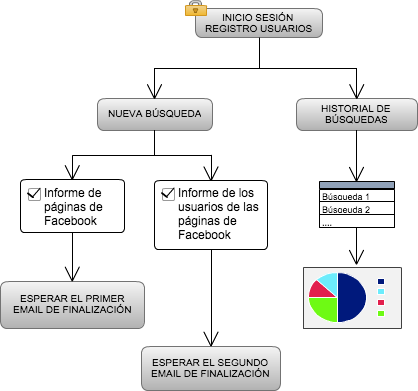
\includegraphics[width=3in]{figuras/appWeb.png}
\caption{Esquema funcionamiento frontend} \label{fig:web}
\end{figure}
Cada una de las pantallas está definida en una vista distinta que se definen a continuación por separado, explicando en detalle cada una de las acciones que el usuario puede realizar. 
\subsection{Registration}
\begin{figure}[H]
\centering
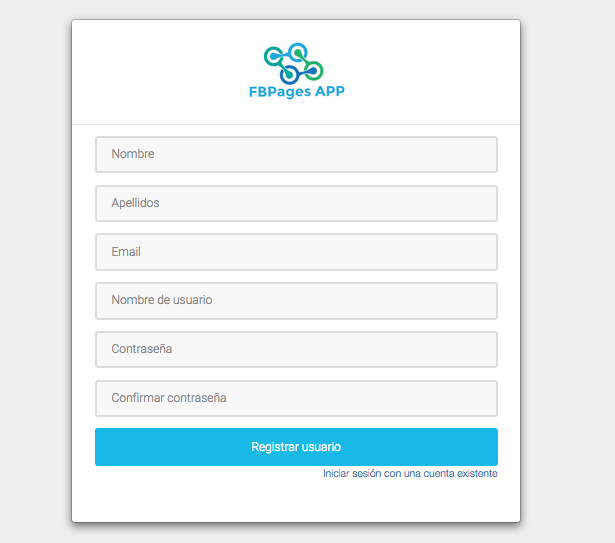
\includegraphics[width=4in]{figuras/registro.png}
\caption{Captura de pantalla del formulario de Registro} \label{fig:registration}
\end{figure}
En esta vista se define un formulario con un objeto de tipo "User", donde el usuario debe introducir todos los datos relacionados con su perfil, para poder crear una cuenta nueva en la aplicación. 

El controlador "RegistrationController.java" se encarga de comprobar que el usuario haya rellenado todos los campos del formulario, y que los datos introducidos sean correctos, en concreto que el campo email, se corresponda con una dirección de correo electrónico, y que la contraseña introducida coincida con la de verificación. 

Si el formulario es correcto, se crea un nuevo usuario que se almacena en la base de datos en la colección "users". 

\subsection{Login}

\begin{figure}[H]
\centering
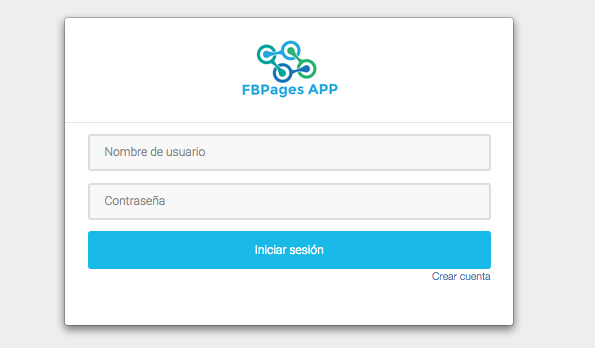
\includegraphics[width=5in]{figuras/login.png}
\caption{Captura de pantalla del formulario de Inicio de Sesión} \label{fig:login}
\end{figure}

En esta vista se presenta el formulario de inicio de sesión del usuario. Para poder acceder a la aplicación se requiere estar previamente registrado. 

De forma similar a la anterior vista, el controlador "LoginController.java" se encarga de que el usuario haya introducido bien el nombre de usuario y la contraseña, de ser así, se conecta con la base de datos y comprueba que exista dentro de la colección "users". Si existe, le da acceso a la aplicación, y si no le indica que no existe el usuario.
\subsection{Búsqueda} \label{sec:4.1.3}

Esta es la pantalla principal de la aplicación, aquí el usuario definirá las características del estudio que quiere realizar. 
Este formulario se define mediante el modelo "Page". Para facilitar la búsqueda al usuario, el formulario se ha dividido en cuatro pasos. Cada paso, está formado por un formulario sencillo, incluyen una breve explicación de los datos que se deben introducir.

A continuación se explica cada uno de los pasos brevemente, los campos necesarios en cada uno y además se muestra su aspecto visual: \\
\\
\begin{itemize} \itemsep4pt \parskip0pt
\item Paso 1/4 \\
\begin{figure}[H]
\centering
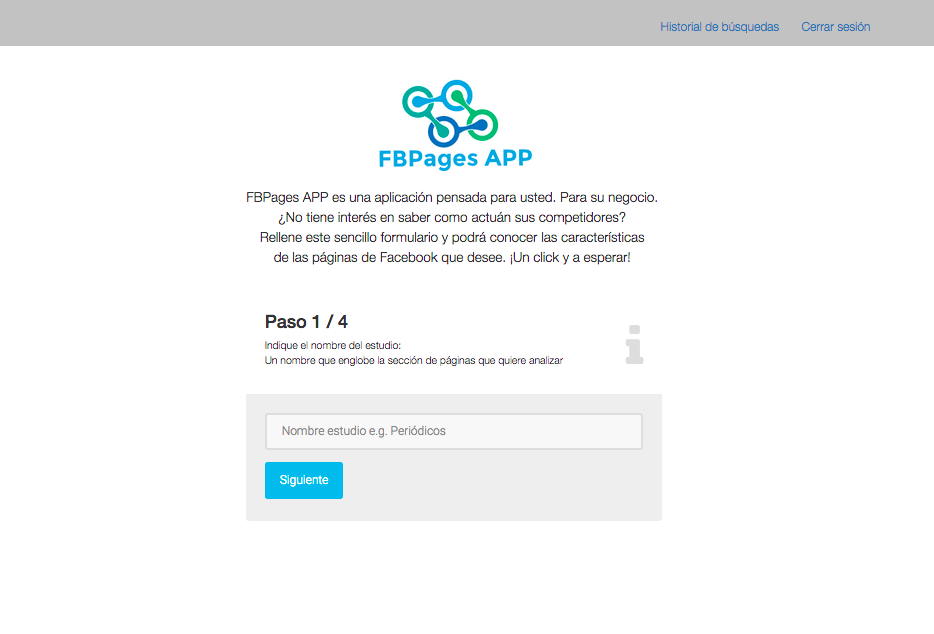
\includegraphics[width=4.5in]{figuras/paso1.png}
\caption{Captura de pantalla del Paso 1} \label{fig:paso1}
\end{figure}
El usuario debe indicar el nombre del estudio que va a realizar
\item Paso 2/4 \\
\begin{figure}[H]
\centering
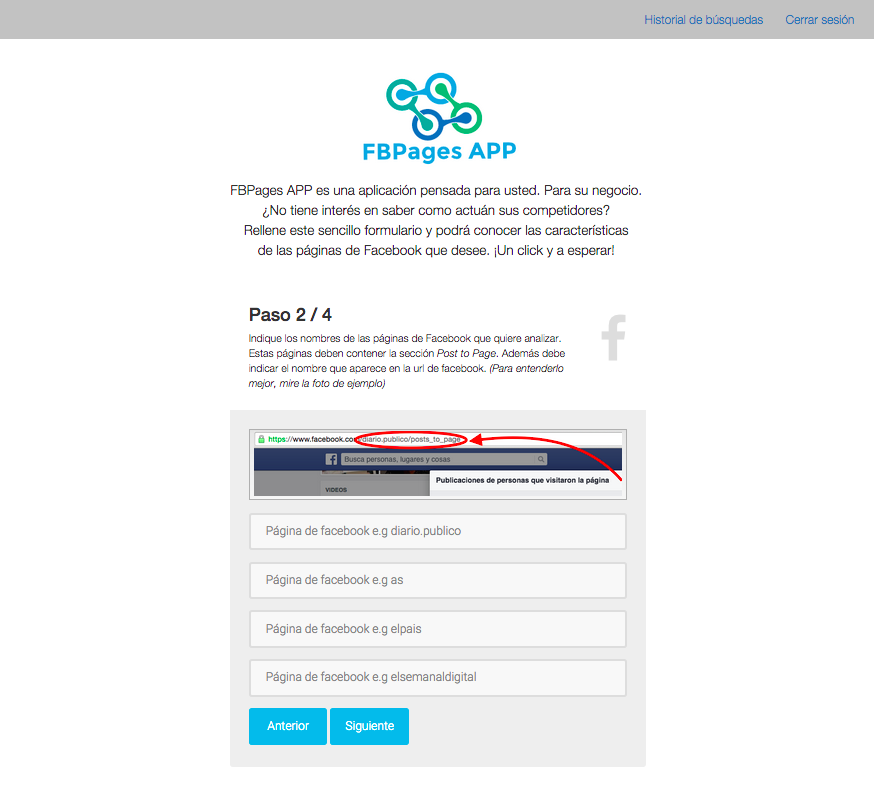
\includegraphics[width=4.5in]{figuras/paso2.png}
\caption{Captura de pantalla del Paso 2} \label{fig:paso2}
\end{figure}
El usuario debe introducir el nombre de las cuatro páginas de Facebook que quiere analizar. Como se puede observar en la figura (\ref{fig:paso2}), se ha introducido una imagen explicativa de la comprobación que debe hacer el usuario antes de añadir una página al formulario, para saber si dicha página contiene la sección \textit{Post To Page}, explicada anteriormente en el presente documento. Si contiene dicha sección, el nombre que debe introducir el usuario en el formulario, es el que aparece en la url de Facebook, para asegurarse de que es la página correcta la que se va a analizar. 
\begin{figure}[H]
\centering
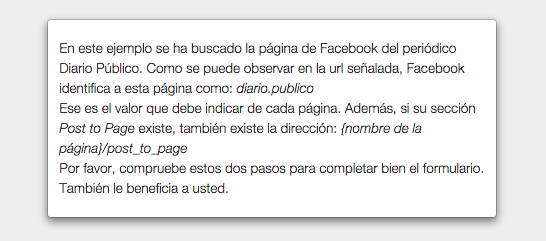
\includegraphics[width=3in]{figuras/help.png}
\caption{Captura de pantalla del diálogo de ayuda del paso 2} \label{fig:hel}
\end{figure}
Este paso es necesario ya que en Facebook existen muchas páginas con nombres similares pero de contenido totalmente opuesto, de esta forma, el usuario se asegura de que la página que se va a analizar es la correcta. 
\item Paso 3/4 \\
\begin{figure}[H]
\centering
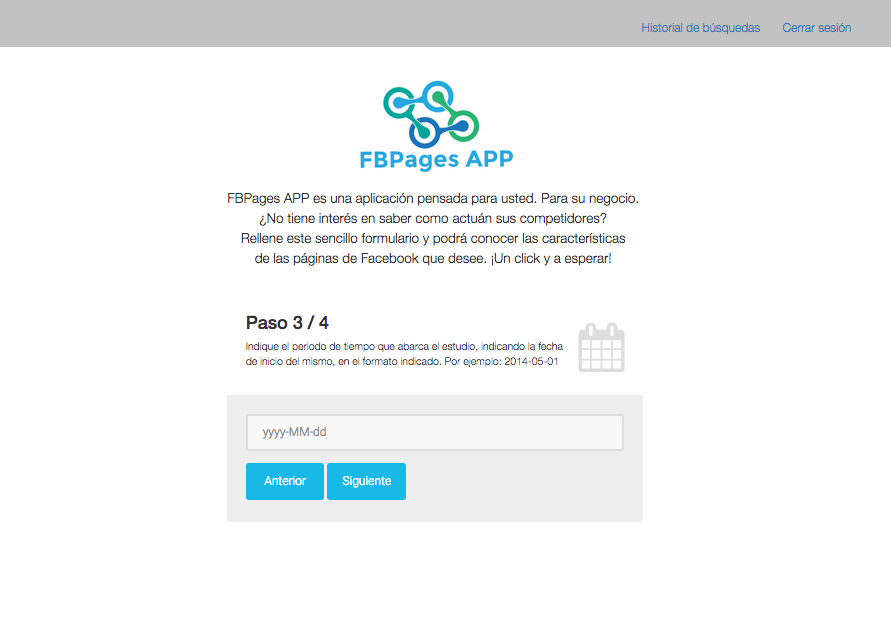
\includegraphics[width=5in]{figuras/paso3.png}
\caption{Captura de pantalla del Paso 3} \label{fig:paso3}
\end{figure}
En este paso el usuario debe indicar la fecha de inicio del estudio. Con este dato, la petición realizada a la API de Facebook se realizará desde la fecha de inicio hasta la fecha actual. Con este dato, el usuario puede decidir si quiere realizar un análisis de las últimas semanas, meses o años. \\
\\
\item Paso 4/4 \\
\begin{figure}[H]
\centering
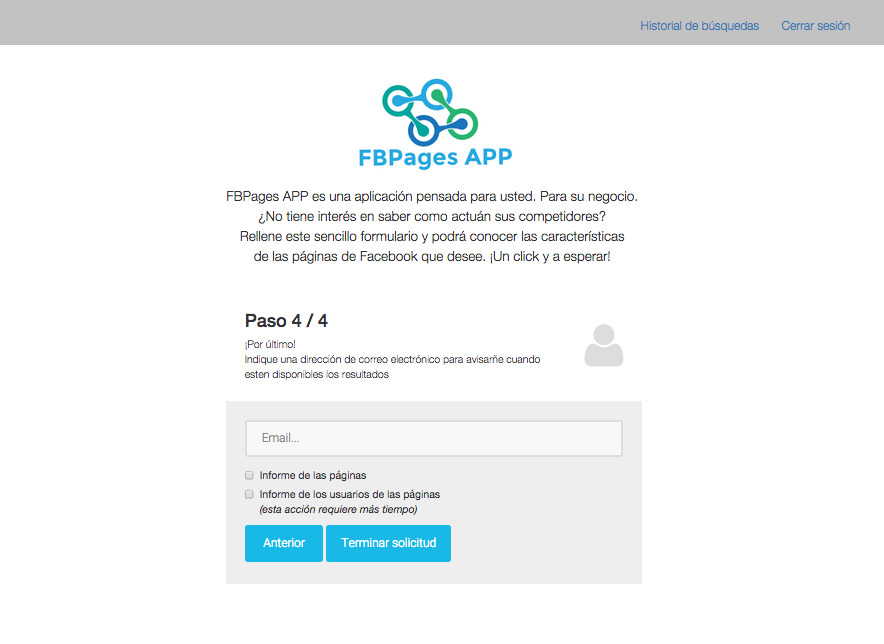
\includegraphics[width=5in]{figuras/paso4.png}
\caption{Captura de pantalla del Paso 4} \label{fig:paso4}
\end{figure}
Por último, el usuario debe indicar la dirección de correo donde quiere que se le avise cuando el estudio haya terminado de recopilar los datos. 
\end{itemize}

Una vez completado el formulario, el controlador "PageController.java" se encarga de almacenar esta búsqueda en la base de datos en la colección "pages", además de incluir los datos de la búsqueda introducidos por el usuario, también se añade al documento de la base de datos el "ID" del usuario, de forma que se pueda relacionar cada búsqueda con su usuario correspondiente. 

Acto seguido, el controlador se encarga de llamar a la siguiente acción. De cara al usuario, aparece una pantalla en la que se le indica que se están recogiendo los datos y que una vez haya acabado este proceso se le enviará un correo electrónico para notificárselo, tal y como se muestra en la siguiente figura (\ref{fig:working}).
\begin{figure}[H]
\centering
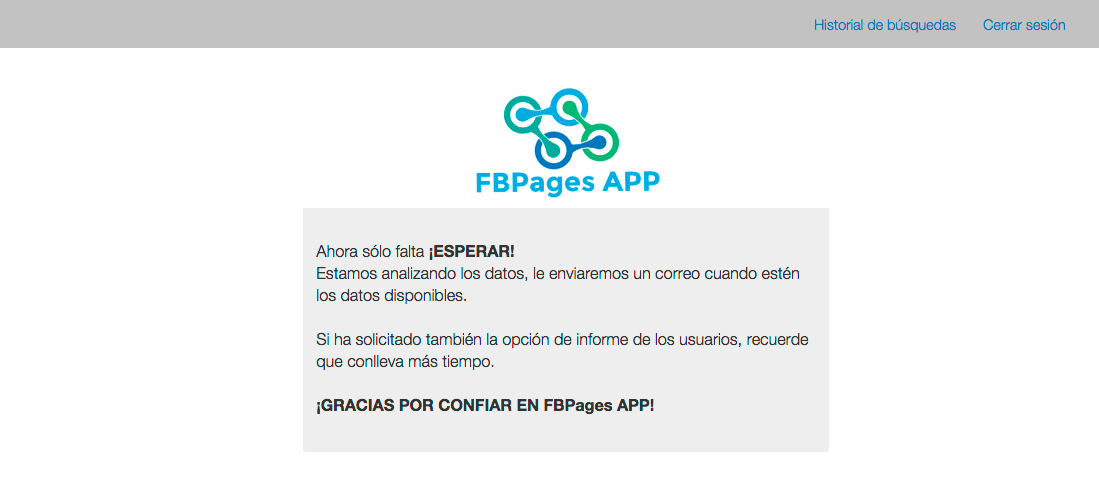
\includegraphics[width=4in]{figuras/working.png}
\caption{Captura de pantalla de la página de espera} \label{fig:working}
\end{figure}
No es tan sencillo como el usuario puede apreciar. Del controlador "PageController.java" se llama al controlador "WorkingController.java". Este controlador lo primero que hace es redirigir la página web a la vista "waiting.jsp" mostrada en la anterior figura. Esta vista está manejada por el controlador "WaitingController.java" que sólo se encarga de mostrar dicha vista. 

Por otro lado, el controlador  "WorkingController.java" inicia una tarea asíncrona. Una tarea asíncrona es aquella que es realiza en segundo plano para no alterar el flujo de la aplicación. 
Para manejar tareas asíncronas en una aplicación web en Spring MVC, se ha creado un \textit{Servlet} asíncrono. 
Un \textit{Servlet} es una clase de lenguaje de programación Java, utilizada para ampliar las capacidades de un servidor. Son utilizados para manejar las páginas web de forma dinámica a partir de los parámetros de la petición que envíe el navegador. Un \textit{Servlet} asíncrono tiene además la función de manejar hilos de tareas que requieren un largo tiempo de espera, de esta forma el navegador no está cargando hasta que se finalice la tarea. 

En la siguiente figura \ref{fig:sa} se muestra el esquema de funcionamiento de un \textit{Servlet} asíncrono. 
\begin{figure}[H]
\centering
\includegraphics[width=4in]{figuras/Servletasincrono.png}
\caption{Ejemplo de funcionamiento de un \textit{Servlet} asíncrono} \label{fig:sa}
\end{figure} 

La tarea asíncrona que maneja este controlador es la conexión con la API de Facebook para sacar los datos de las páginas solicitadas, esta función se explica en detalle más adelante en la sección (\ref{sec:4.2.2}). 

Una vez completada esta tarea, el controlador realiza dos pasos. Por un lado, envía un correo electrónico al usuario para notificarle que el estudio de las páginas de Facebook ha terminado, enviando el enlace donde puede acceder para ver los resultados. Por otro lado, envía un correo al administrador de la aplicación, en este caso la propia autora del trabajo fin de grado, para indicar que se ha solicitado el estudio de usuarios de las páginas, esta parte del proyecto se ha definido así porque el \textit{crawler} requiere ciertos servicios que deben estar correctamente activados antes de lanzarlo automáticamente, el funcionamiento de esta parte se explica más adelante en el sección (\ref{sec:4.2.3}).

\subsection{Historial}
\begin{figure}[H]
\centering
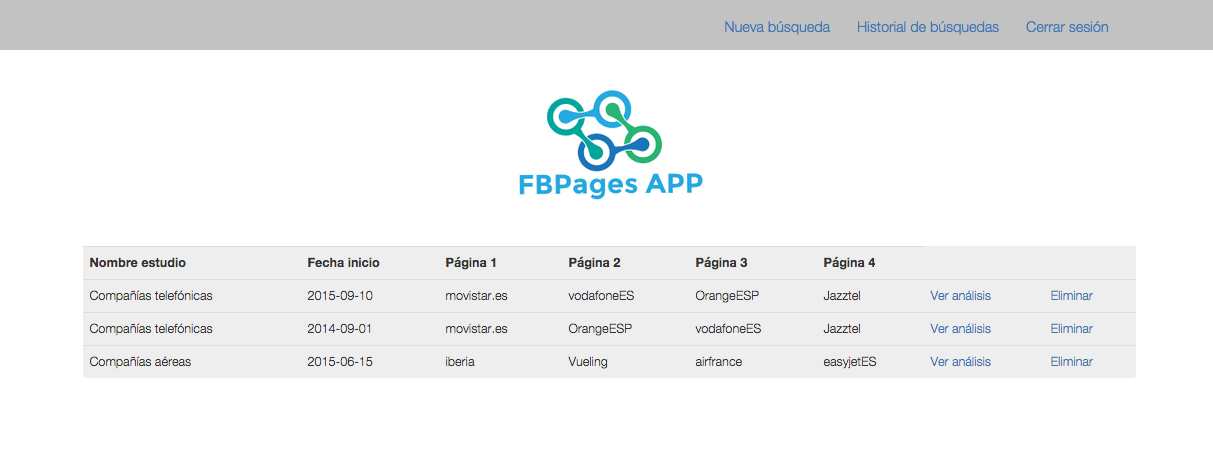
\includegraphics[width=5in]{figuras/historial.png}
\caption{Captura de pantalla de la página Historial} \label{fig:historial}
\end{figure}
Otra de las funciones a las que tiene acceso el usuario es a ver todos los estudios que ha solicitado en la aplicación. Esta vista muestra una tabla con todos los datos relacionados con el usuario. Desde esta tabla el usuario tiene dos acciones: "Ver el análisis" del estudio que elija o "Eliminar" esa búsqueda. 

Internamente el controlador "HistoryController.java" solicita a la base de datos "pages" que le devuelva todos los objetos que contienen el "ID" de usuario que corresponden con el que ha iniciado sesión en la aplicación, y devuelve la lista de páginas a la vista que se renderiza en la tabla que se observa en la figura (\ref{fig:historial}).

Además, si el usuario pulsa en la opción "Ver análisis", el controlador redirecciona la página a la vista "graphs.jsp" que es la encargada de mostrar los gráficos diseñados para la búsqueda seleccionada. 

Si por el contrario el usuario selecciona la opción "Eliminar", el controlador mediante una operación sencilla del CRUD definido para las páginas, eliminará esa entrada de la base de datos.
 
\subsection{Resultados} \label{sec:4.1.5}
Por último, la vista que muestra los resultados de un estudio concreto. Los usuarios pueden acceder a esta vista pulsando en el link que se les envía por correo electrónico o desde el historial, pulsando en la opción "Ver análisis". Pulsando en dicha opción, el usuario vería la siguiente pantalla que se muestra en la siguiente figura (\ref{fig:resultados})
\begin{figure}[H]
\centering
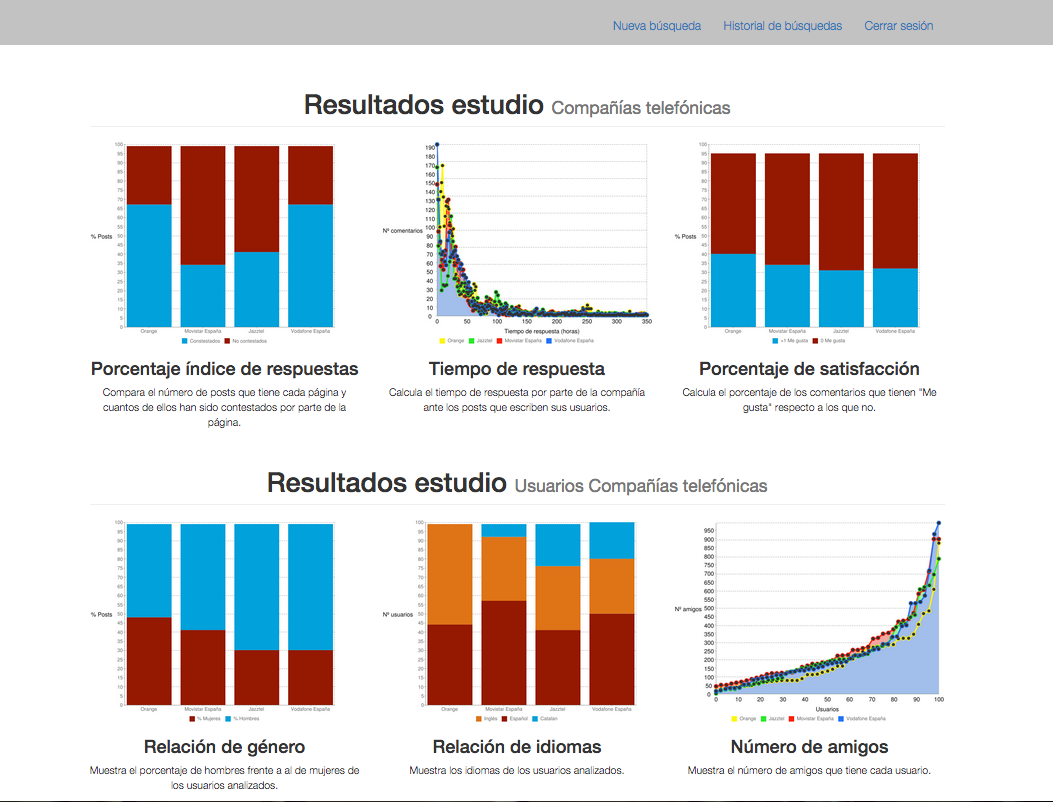
\includegraphics[width=5in]{figuras/ejemploCompleto.png}
\caption{Captura de pantalla del resultado del análisis} \label{fig:resultados}
\end{figure}

Esta vista se maneja por el controlador "ChartController.java". Se encarga de procesar los datos recogidos en la base de datos de MySQL con el nombre concreto de la búsqueda y los representa en gráficas mediante Google Chart. 

Google Chart es un herramienta para desarrolladores que permite la creacción de gráficas en forma de imágenes PNG para poder utilizarlas en las páginas web. Para utilizar esta herramienta se ha utilizado una librería de java "charts4j" \cite{charts} que permite integrar las funcionalidades de Google Chart en la aplicación. 

Se han definido las gráficas por defecto, lo único que cambian son los datos que las definen, que son cogidos de la base de datos. En el siguiente listado se muestran todas las gráficas que se han realizado y un ejemplo de cada una de ellas: 
\begin{enumerate}
\item \textbf{ESTUDIO BASADO EN LAS PÁGINAS DE FACEBOOK}
\begin{itemize}
\item \textbf{Porcentaje índice de respuesta}\\
\begin{figure}[H]
\centering
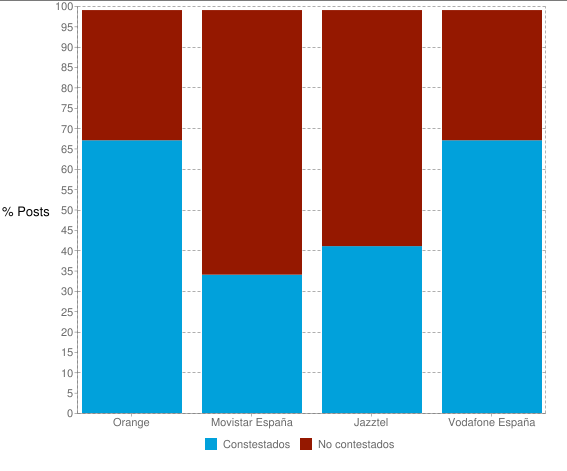
\includegraphics[width=2in]{figuras/contestados.png}
\caption{Gráfica porcentaje índice de respuesta} \label{fig:contestados}
\end{figure}
Esta gráfica presenta los resultados de los datos obtenidos, obteniendo el porcentaje del total de los comentarios que ha contestado la página bajo estudio frente a los que no.  

\item \textbf{Tiempo de respuesta}\\
\begin{figure}[H]
\centering
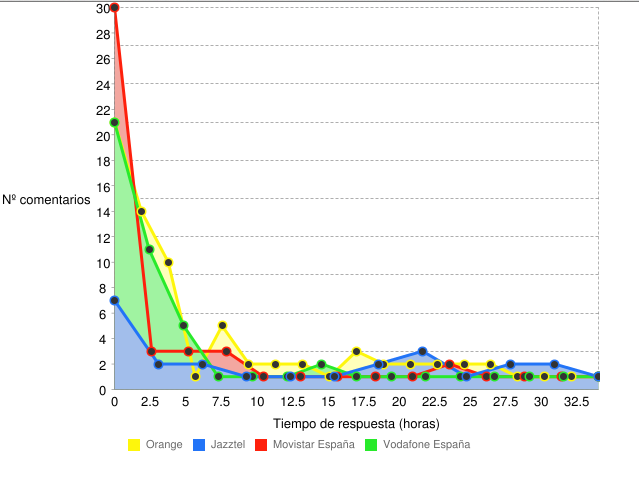
\includegraphics[width=2in]{figuras/tiempo.png}
\caption{Gráfica tiempo de respuesta} \label{fig:tiempo}
\end{figure}
Esta gráfica muestra el tiempo de respuesta por parte de la página a los comentarios que escriben los usuarios. Este tiempo está calculado en horas.
\item \textbf{Porcentaje de satisfacción}\\
\begin{figure}[H]
\centering
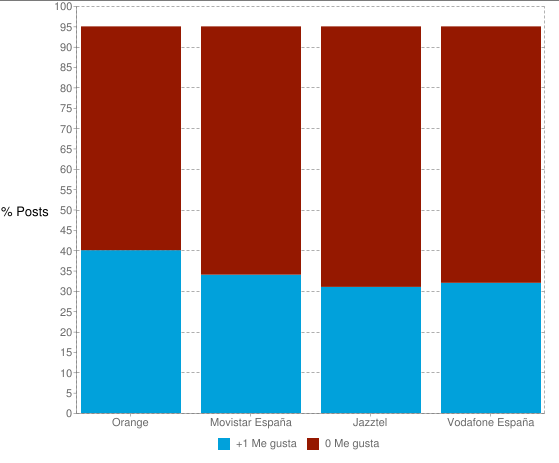
\includegraphics[width=2in]{figuras/satisfaccion.png}
\caption{Gráfica porcentaje de satisfacción} \label{fig:satisfaccion}
\end{figure}
Este gráfico representa el porcentaje de comentarios que han obtenido algún "Me gusta" (\textit{Likes}, comúnmente conocido) frente a los que no. 
\end{itemize}
\item \textbf{ESTUDIO BASADO EN LOS USUARIO DE LAS PÁGINAS DE FACEBOOK}
\begin{itemize}
\item \textbf{Relación de género}\\
\begin{figure}[H]
\centering
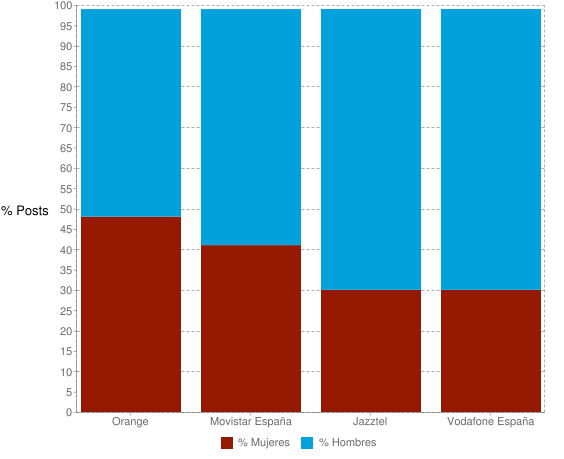
\includegraphics[width=2in]{figuras/genero.png}
\caption{Gráfica relación de genero} \label{fig:genero}
\end{figure}
Esta gráfica muestra el porcentaje de hombres y mujeres dentro de los usuarios analizados de cada página.  
\item \textbf{Relación de idiomas}\\
\begin{figure}[H]
\centering
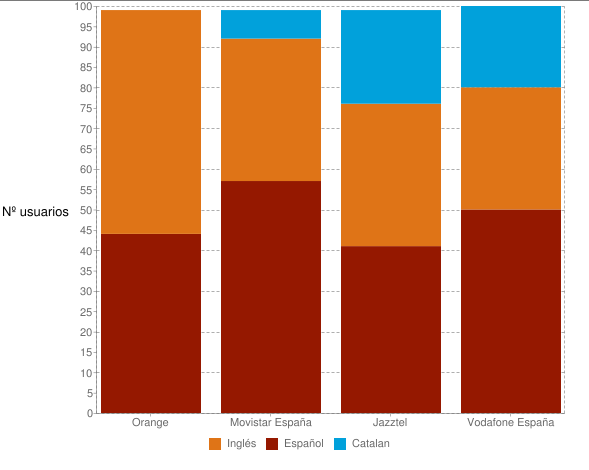
\includegraphics[width=2in]{figuras/idioma.png}
\caption{Gráfica relación de genero} \label{fig:idioma}
\end{figure}
Esta gráfica representa el porcentaje de usuarios de habla ingles, española o catalana. Aunque no es un dato muy fiable, dado que muchos usuarios dominarán más del idioma materno, por norma general, aquellos usuarios que especifican un idioma, indican su propia lengua materna.
\item \textbf{Número de amigos}\\
\begin{figure}[H]
\centering
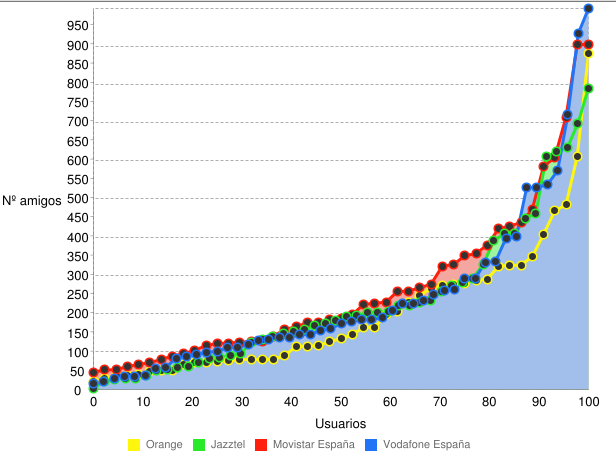
\includegraphics[width=2in]{figuras/amigos.png}
\caption{Gráfica número de amigos} \label{fig:amigos}
\end{figure}
En esta gráfica se muestra el número de amigos que tiene cada uno de los usuarios analizados. El fin de esta gráfica es considerar si son cuentas activas o no, ya que si el porcentaje de usuarios con cero amigos es muy elevado, podría indicar que son usuarios falsos.
\end{itemize}
\end{enumerate}

\section{Backend}
En el lado del servidor tenemos una estructura más compleja, que se va a explicar dividiéndolo en cada una de las herramientas utilizadas o creadas para el correcto funcionamiento de la aplicación.
Primeramente, se va a mostrar el diagrama completo del backend, tal y como se muestra en la figura (\ref{fig:backend}). 
\begin{figure}[H]
\centering
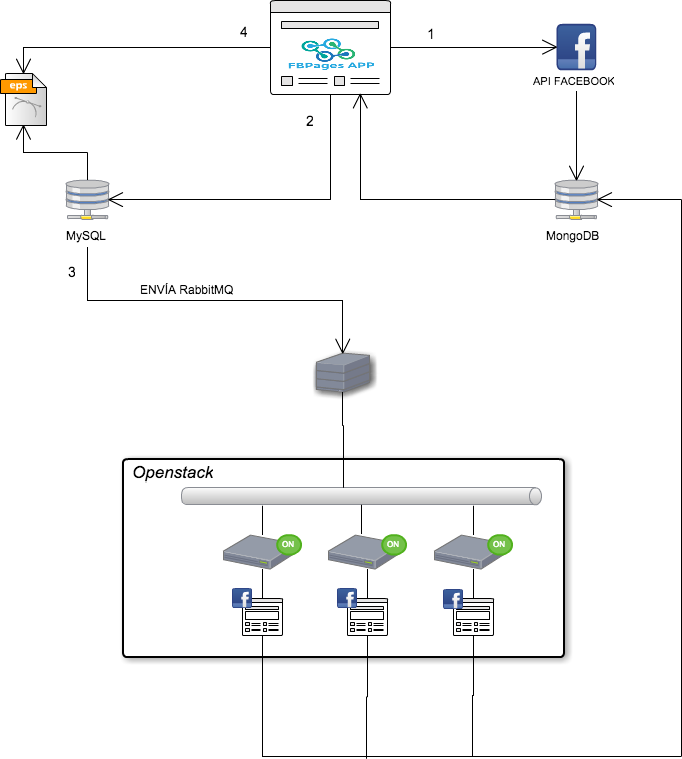
\includegraphics[width=4in]{figuras/backend.png}
\caption{Esquema funcionamiento backend} \label{fig:backend}
\end{figure}

Como se puede observar en la anterior figura, hay varios pasos implementados, que tienen que seguir el orden indicado para poder obtener todos los datos requeridos.

\subsection{API Facebook Developers} \label{sec:4.2.2}
El primer paso indicado es la API de Facebook. El usuario en la aplicación indicará los datos necesarios para realizar la consulta a la API, una vez obtenidos esos datos por parte del usuario, se lanza un script, de manera asíncrona, tal y como se ha explicado en la sección (\ref{sec:4.1.3}). En este punto se va a explicar más en detalle como funciona este programa.

La API de Facebook es la principal forma de obtener los datos dentro y fuera del gráfico social de Facebook. Es una API basada en HTTP que se ha utilizado para consultar datos. A continuación se muestra un ejemplo de una petición a la API de Facebook, mediante su herramienta \textit{Graph API}. Esta herramienta permite ver los resultados de la consulta que se desea hacer. 
\begin{figure}[H]
\centering
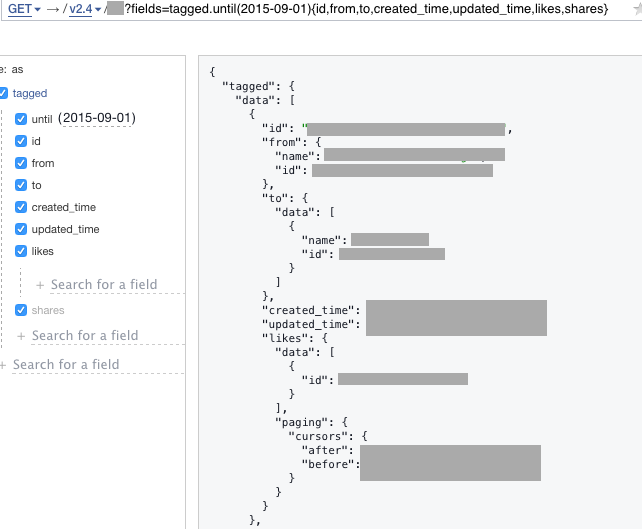
\includegraphics[width=4in]{figuras/ejemploAPI.png}
\caption{Esquema petición API Facebook} \label{fig:ejemploAPI}
\end{figure}

Para poder obtener los datos de las páginas de Facebook indicadas por el usuario de forma automática, se ha creado un programa que realiza las peticiones a la API de Facebook con los parámetros necesarios, en nuestro caso de la sección \textit{tagged}, que se corresponde con los posts de los usuarios en las páginas. 

La API de Facebook devuelve en formato JSON los resultados, este fichero es almacenado directamente en la base de datos de MongoDB, para su posterior procesado.

Esta acción se repite para cada una de las páginas indicadas por el usuario, hasta completar la obtención de datos necesaria. 

El segundo paso consiste en leer los datos obtenidos y almacenados en MongoDB, coger sólo aquellos datos de interés para este trabajo fin de grado y ordenarlos en una tabla en MySQL. De esta forma, es más fácil acceder a ellos y representarlos.

\subsection{Distribución: RabbitMQ}
Una vez guardados los datos en MySQL, si el usuario ha seleccionado la opción de "Informe de los usuarios de las páginas", el siguiente paso es lanzar el \textit{crawler} para recoger los datos de los usuarios. 

Antes de explicar el funcionamiento del \textit{crawler}, se va a explicar la arquitectura desplegada mediante RabbitMQ para la correcta distribución del \textit{crawler}. Como se ha explicado en el Estado del Arte, RabbitMQ es un sistema de intercambio de mensajes. La utilización en este trabajo fin de grado se basa en el envío de mensajes a cuatro máquinas virtuales en las que se ejecutará el \textit{crawler}. 

El sistema es muy sencillo, se configuran las cuatro máquinas virtuales con el entorno necesario para ejecutar el \textit{crawler}. Una vez hecho esto, se lanza el script de RabbitMQ que tiene la función de recibir. Cada VM recibe mensajes de una cola de mensajes distinta, por lo que el emisor es el encargado de decidir que envía a cada VM, o lo que es lo mismo a cada cola. 

Por otro lado, desde la aplicación se maneja el script encargado de enviar los mensajes. Este script manda un mensaje a cada una de las colas de mensajes activas indicando el número de usuarios a analizar y el nombre de la página de donde han sido extraídos. Una vez enviado el mensaje, se queda esperando para recibir la confirmación de que el trabajo ha finalizado. De esta forma, se distribuye el \textit{crawler} en cada máquina virtual de forma automática, sin necesidad de ir a cada una de las VMs para lanzar el \textit{crawler}.

\subsection{Crawler de Facebook: Selenium WebDriver} \label{sec:4.2.3}

El \textit{crawler} es un script escrito en Java, que tiene como función principal recoger los datos de un usuario de Facebook. Se basa en reproducir los pasos que haría un humano si mirase el perfil de un usuario en Facebook. 

Este \textit{crawler} funciona lanzando una instancia del navegador Firefox,  indicando la url de Facebook. Como toda persona que pertenece a esta comunidad, lo primero que debe hacer es iniciar sesión con una cuenta existente, y una vez dentro, procede a visitar los perfiles de cada uno de los usuarios que se le han indicado. El número de usuarios estipulado para este proyecto han sido 100, número suficiente para poder perfilar los patrones de los usuarios más comunes de una página web.

La instancia que lanza en navegador recibe el nombre de WebDriver, permite configurar y ejecutar los comandos necesarios para parsear la web y coger los datos deseados. 

Los datos recogidos de los usuarios en Facebook, son almacenados de igual forma que los de la API de Facebook, se crea un objeto JSON con todos los campos obtenidos del perfil y se almacena directamente en MongoDB. Se ha definido de esta forma por si en un futuro cambian los campos del perfil de un usuario de Facebook, añadiendo o eliminando algún campo, solo habría que modificar el fichero JSON que se va a introducir en la base de datos, sin necesidad de modificar nada más. 

\subsection{Análisis gráfico: Google Chart}

Por último, el cuarto paso consiste en analizar todos los datos obtenidos tanto de la API de Facebook como del \textit{crawler} para representarlos gráficamente y que el usuario pueda verlo en la interfaz de la aplicación. 

Para representar los datos se ha utilizado la herramienta de Google Chart, que facilita la integración de las gráficas con una aplicación web. Esta herramienta es utilizada en este proyecto mediante una librería de java, ya comentada anteriormente en la sección (\ref{sec:4.1.5}). Se define el tipo de gráfica que se quiere representar, y se le pasa como parámetro los datos ya procesados, Google Chart se encarga de dibujarlos en las gráficas.

Hay dos grandes bloques de datos que se han almacenado en la base de datos para ser procesados, los de los usuarios y los de las páginas de Facebook. 

Por un lado, los datos relacionados con los usuarios, extraídos mediante el \textit{crawler}. De estos datos se obtiene la información de los usuarios en relación a su género, número de amigos e idiomas hablados y se calcula el porcentaje de cada una de las variables para cada página. Una vez calculados los porcentajes, se representan en una tabla conjunta para ver la diferencia de porcentaje entre cada página. 

Por parte de los datos obtenidos de la API de Facebook se han tenido en cuenta la fecha de creación de un mensaje y la fecha de actualización del mismo, si no existe la fecha de actualización significa que la página de Facebook no ha contestado al comentario, y si por el contrario existe, se calcula la diferencia de tiempo, pudiendo así obtener el tiempo de respuesta de la página de Facebook ante un comentario. Con estos dos datos, se obtienen las gráficas del porcentaje de respuesta y del tiempo de respuesta explicadas en la sección (\ref{sec:4.1.5}). También se extrae el dato de número de "Me gusta" que tiene cada comentario para calcular el porcentaje de satisfacción de los usuarios ante las publicaciones recogidas. 

\chapter{Ejemplo de utilización de la aplicación}

Para mostrar el funcionamiento de este trabajo fin de grado gráficamente, a continuación se explica el ejemplo de un caso práctico con todos los pasos seguidos y los resultados obtenidos. 

\section{Caso práctico}

Se supone un usuario que va a solicitar un estudio sobre cuatro páginas de Facebook relacionadas con compañías telefónicas.

\begin{itemize}
\item \textbf{PASO 1: Registro en la aplicación}\\
Se registra en la aplicación como un nuevo usuario. Se llama usuarioPrueba. En la siguiente figura se muestra este paso una vez completado y creado satisfactoriamente.
\begin{figure}[H]
\centering
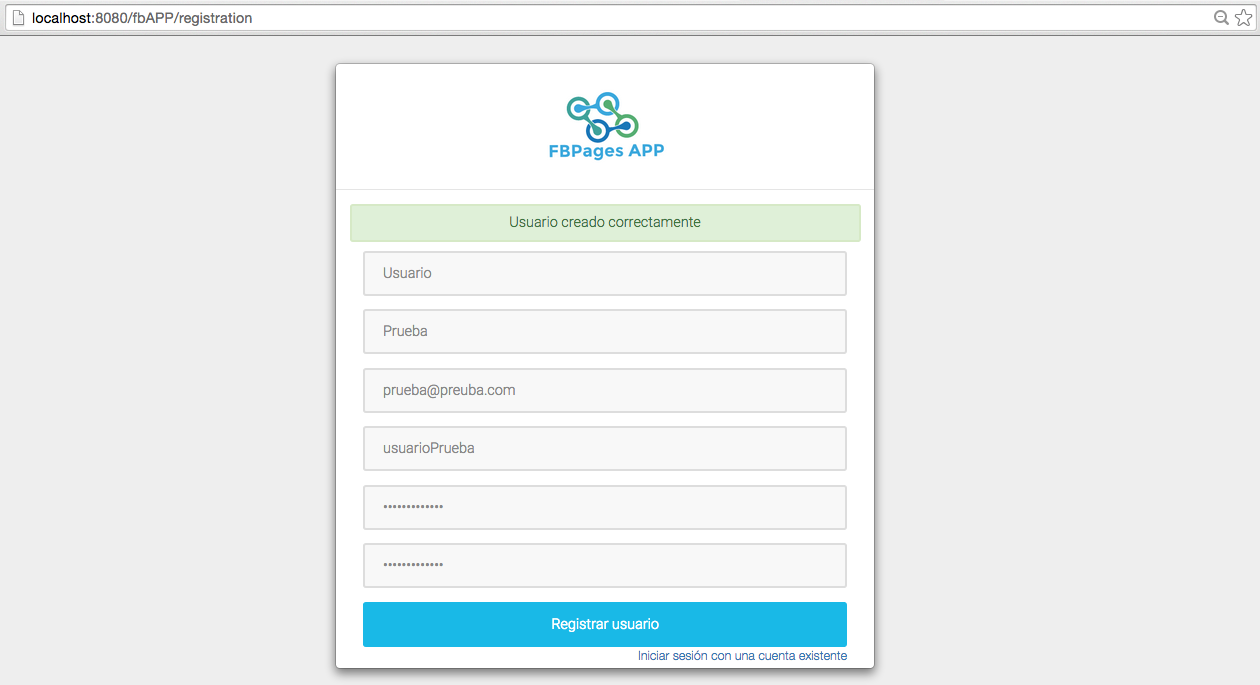
\includegraphics[width=5.5in]{figuras/ejemploRegistro.png}
\caption{Captura de pantalla ejemplo Registro de usuario} \label{fig:exregistro}
\end{figure}
\item \textbf{PASO 2: Inicio de sesión}\\
Una vez creado el usuario, ya puede acceder a la aplicación con el nombre de usuario y contraseña establecidos. A continuación se presenta un ejemplo de este paso gráficamente. 
\begin{figure}[H]
\centering
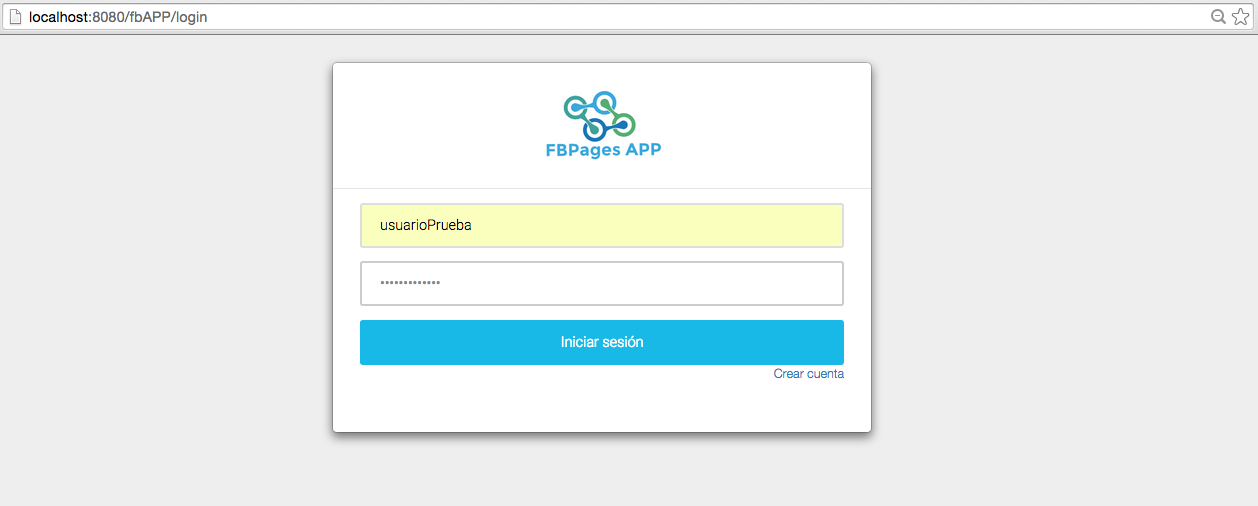
\includegraphics[width=5in]{figuras/ejemploLogin.png}
\caption{Captura de pantalla ejemplo Inicio de sesión} \label{fig:exlogin}
\end{figure}
\item \textbf{PASO 3: Solicitud del análisis a realizar}
El siguiente paso se divide en cuatro. Consiste en definir las características del análisis de que va a realizar.
\begin{enumerate}
\item En el primer formulario hay que indicar el nombre que va a englobar el estudio. En este caso, Compañías telefónicas. 
\begin{figure}[H]
\centering
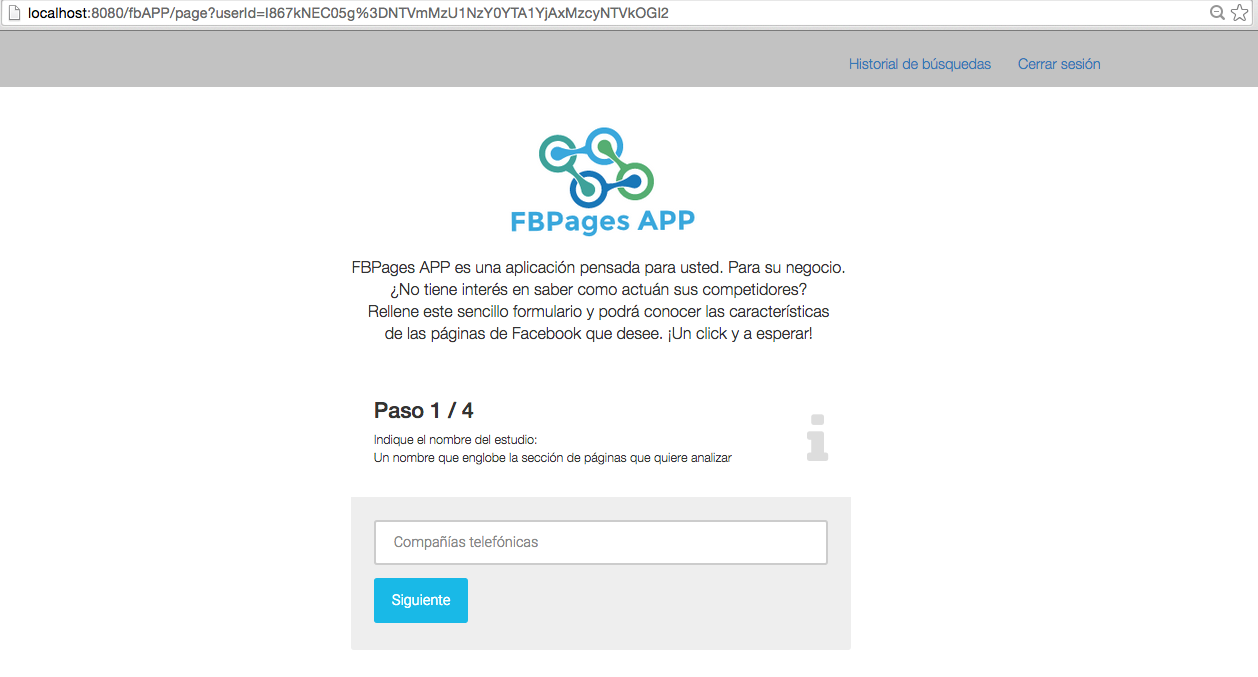
\includegraphics[width=5in]{figuras/ejemploPaso1.png}
\caption{Captura de pantalla ejemplo solicitud de análisis. Paso 1} \label{fig:exPaso1}
\end{figure}
\item En el segundo hay que indicar el nombre de las páginas de Facebook que se van a analizar. En este caso práctico, se quien analizar las páginas de las compañías telefónicas Movistar, Orange, Vodafone y Jazztel. 

No es suficiente con poner el nombre de la compañía, hay que introducir el nombre que Facebook indica en la dirección URL. Para ello, se ha buscado la página de Movistar, a modo de ejemplo. Como es una compañía internacional, hay varias páginas posibles para esta búsqueda, en este caso, se va a elegir Movistar España.  En la siguiente figura se muestra la búsqueda en Facebook para entenderlo mejor.
\begin{figure}[H]
\centering
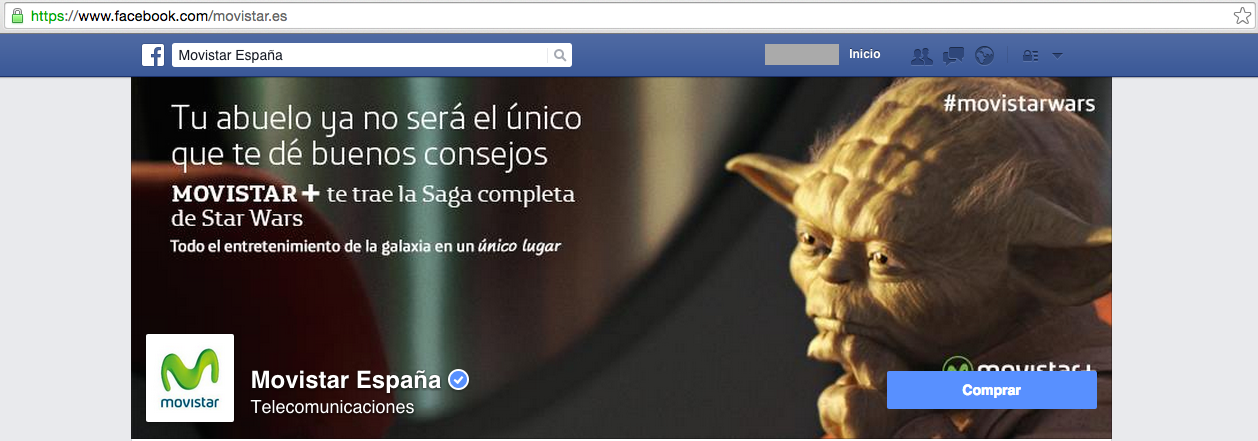
\includegraphics[width=5in]{figuras/ejemploFacebook.png}
\caption{Captura de pantalla ejemplo búsqueda en Facebook} \label{fig:exFacebook}
\end{figure}
Además de elegir la página adecuada para los requisitos esperados del estudio, es conveniente comprobar que existe la sección \textit{Post to Page} de la página seleccionada. Este paso se realiza añadiendo al final de la URL el texto "/posts\_to\_page", y si se carga una pantalla mostrando las publicaciones de los usuarios, significa que existe. A continuación se muestra gráficamente.
\begin{figure}[H]
\centering

\includegraphics[width=5in]{figuras/ejemploPostToPage.png}
\caption{Captura de pantalla ejemplo comprobación sección \textit{Post to Page}} \label{fig:exPostToPage}
\end{figure}
Una vez realizadas las comprobaciones necesarias para las cuatro compañías telefónicas se introducen con el nombre adecuado en el formulario, tal y como se muestra en la siguiente figura.
\begin{figure}[H]
\centering
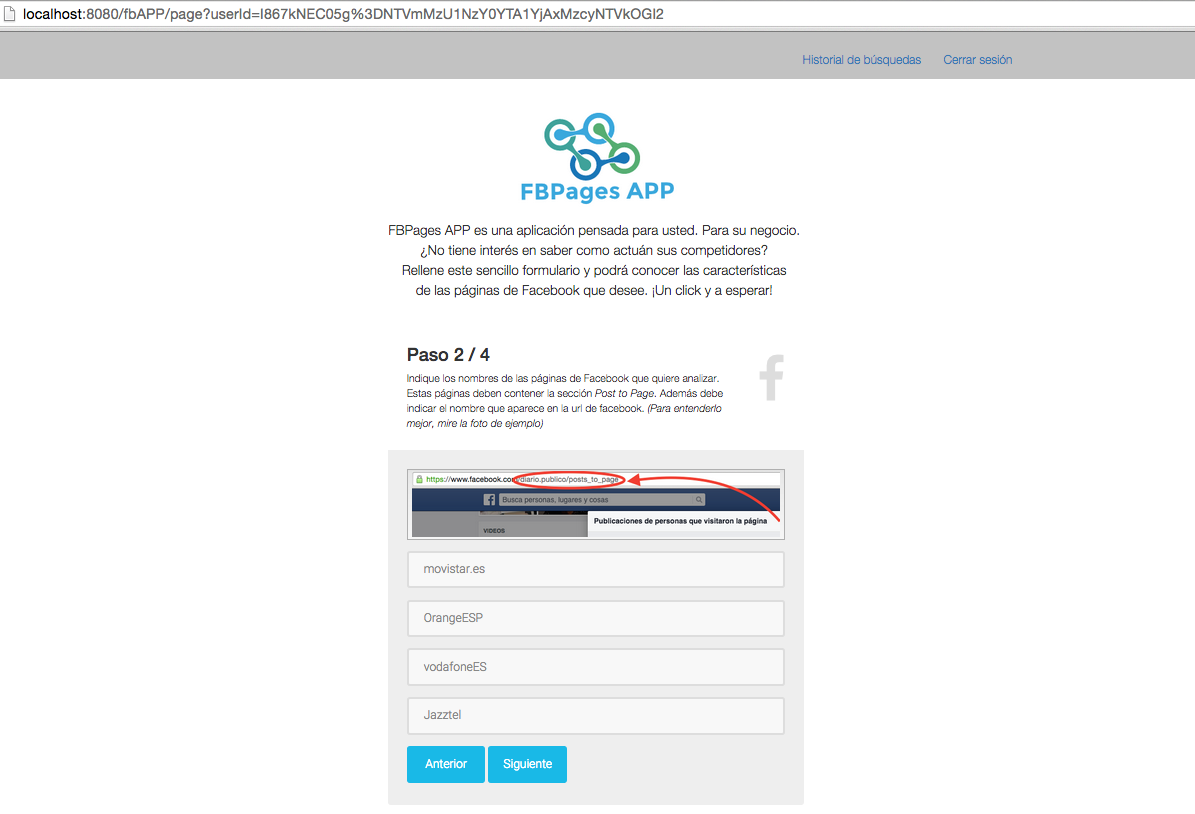
\includegraphics[width=5in]{figuras/ejemploPaso2.png}
\caption{Captura de pantalla ejemplo solicitud de análisis. Paso 2} \label{fig:exPaso2}
\end{figure}
\item En el tercer paso, hay que indicar el periodo temporal del estudio a realizar. En concreto se quiere realizar del último año, por lo que se introducirá la fecha de inicio el uno de septiembre de 2014, en el formato indicado por la aplicación.
\begin{figure}[H]
\centering
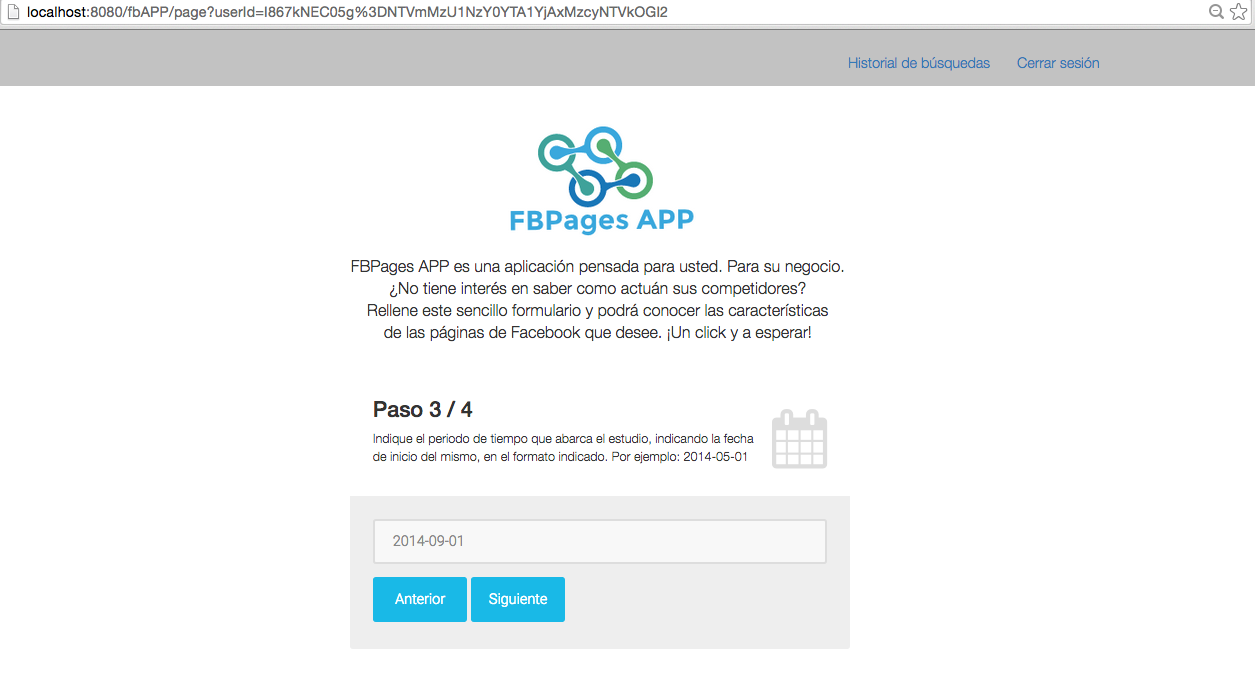
\includegraphics[width=5in]{figuras/ejemploPaso3.png}
\caption{Captura de pantalla ejemplo solicitud de análisis. Paso 3} \label{fig:exPaso3}
\end{figure}
\item Por último, se debe indicar una dirección de correo electrónico a la que se avisará una vez finalizado el estudio de Facebook, además de seleccionar las características del análisis. En este caso se van a seleccionar ambas, "Informe de las páginas" e "Informe de los usuarios de las páginas". 
\begin{figure}[H]
\centering
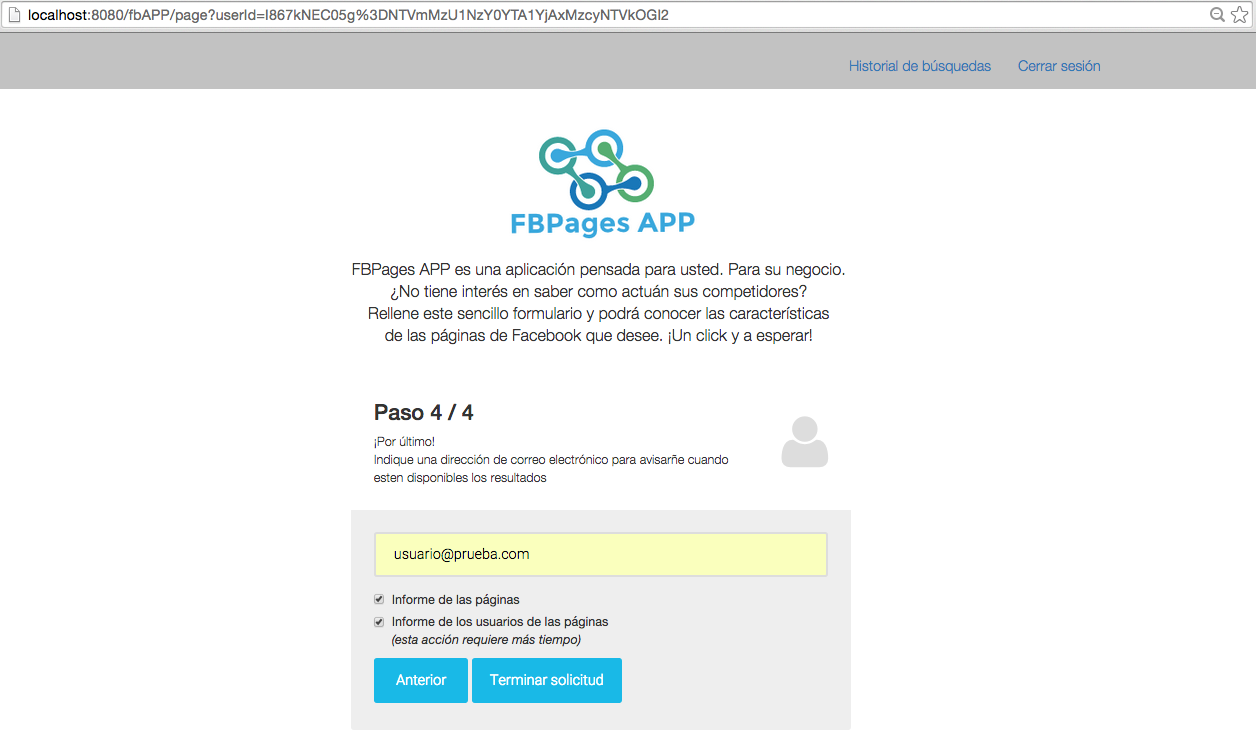
\includegraphics[width=5in]{figuras/ejemploPaso4.png}
\caption{Captura de pantalla ejemplo solicitud de análisis. Paso 4} \label{fig:exPaso4}
\end{figure}
Una vez completados todos los formularios necesarios para realizar una solicitud de un análisis, se pulsa en el botón "Terminar solicitud".
\end{enumerate}
\item \textbf{PASO 4: Tiempo de espera hasta que llegue la notificación por correo}\\
Después de pulse el botón "Terminar solicitud", se visualiza la pantalla que se muestra a continuación. En la que se indica al usuario que debe esperar a que se haya realizado el análisis de las páginas de Facebook.
\begin{figure}[H]
\centering
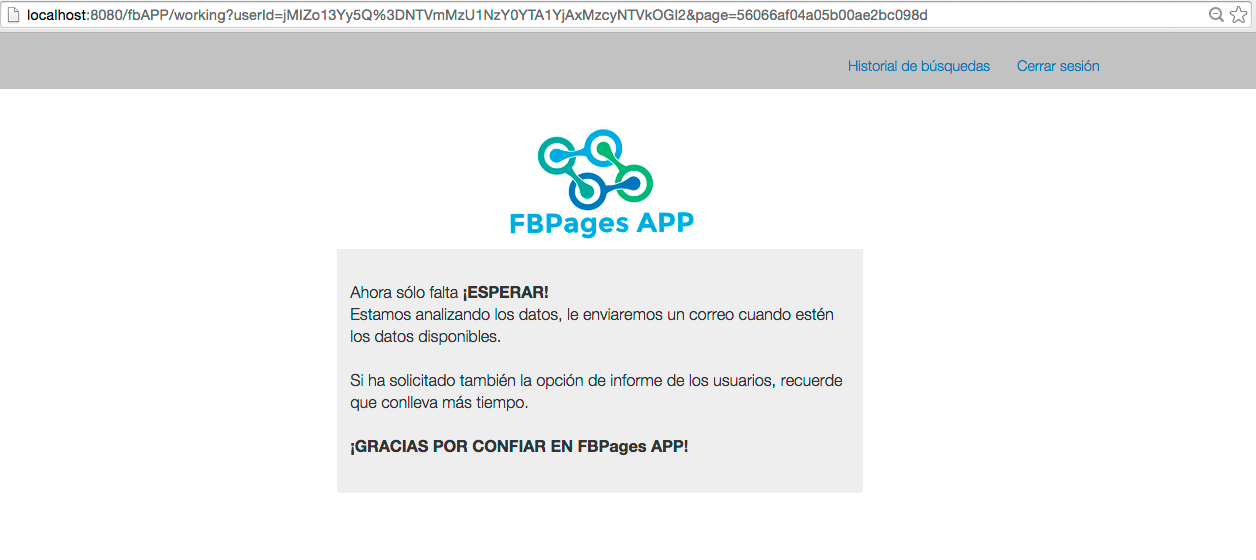
\includegraphics[width=5in]{figuras/ejemploWorking.png}
\caption{Captura de pantalla ejemplo pantalla de espera} \label{fig:exWorking}
\end{figure}

Pasado el tiempo necesario para obtener los datos del análisis, el usuario recibe un correo donde se le avisa de que ya puede ver los resultados del estudio. En la siguiente imagen, se muestra un ejemplo del correo recibido.

\begin{figure}[H]
\centering
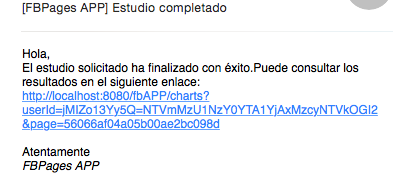
\includegraphics[width=5in]{figuras/ejemploCorreo.png}
\caption{Captura de pantalla ejemplo correo recibido} \label{fig:exCorreo}
\end{figure}

\item \textbf{PASO 5: Visualización de los resultados}
Pinchando en el enlace indicado en el correo recibido (Figura \ref{fig:exCorreo}) se pueden ver los resultados. Otra opción es acceder de nuevo a la aplicación y pulsar sobre la opción "Historial de búsquedas", donde aparece una tabla que recoge todos los análisis solicitados y se selecciona la opción "Ver análisis". En la siguiente figura se muestra el Historial de Búsquedas del usuarioPrueba. 
\begin{figure}[H]
\centering
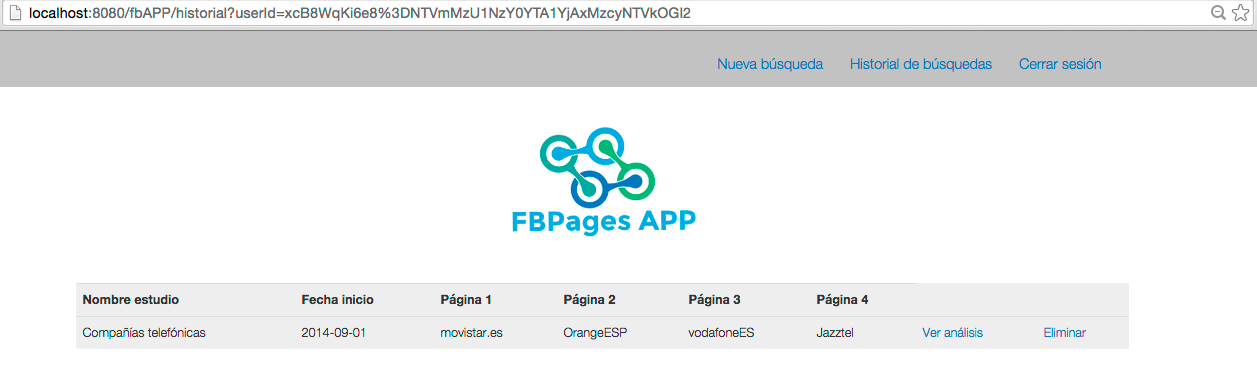
\includegraphics[width=5in]{figuras/ejemploHistorialUser.png}
\caption{Captura de pantalla ejemplo historial de búsquedas del usuario} \label{fig:exHistorial}
\end{figure}

Por último, para finalizar la explicación de este caso práctico, se presentan los resultados que ha obtenido el usuario después de todo el proceso.

Dado que el análisis de los usuarios requiere más tiempo, si el usuario accede automáticamente después de recibir el correo, sólo ve el análisis de las páginas de Facebook, y el análisis de los usuarios en espera. Tal y como se muestra en la siguiente figura. 
\begin{figure}[H]
\centering
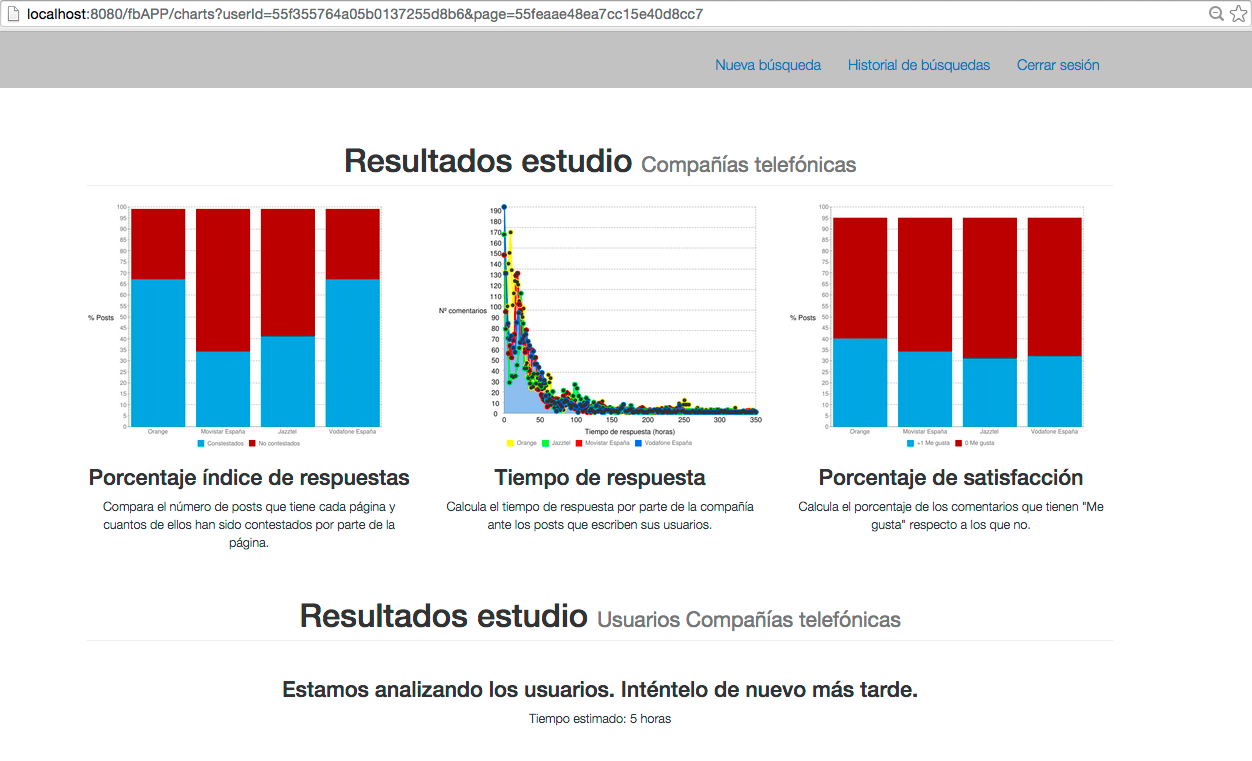
\includegraphics[width=5in]{figuras/ejemploAnalisisFB.png}
\caption{Captura de pantalla ejemplo análisis obtenido. Sólo las páginas} \label{fig:exAnalisisFB}
\end{figure}
Si transcurrido un tiempo vuelve a acceder a la aplicación, ya estarán disponibles los resultados de los usuarios, visualizando el análisis completo.
\begin{figure}[H]
\centering
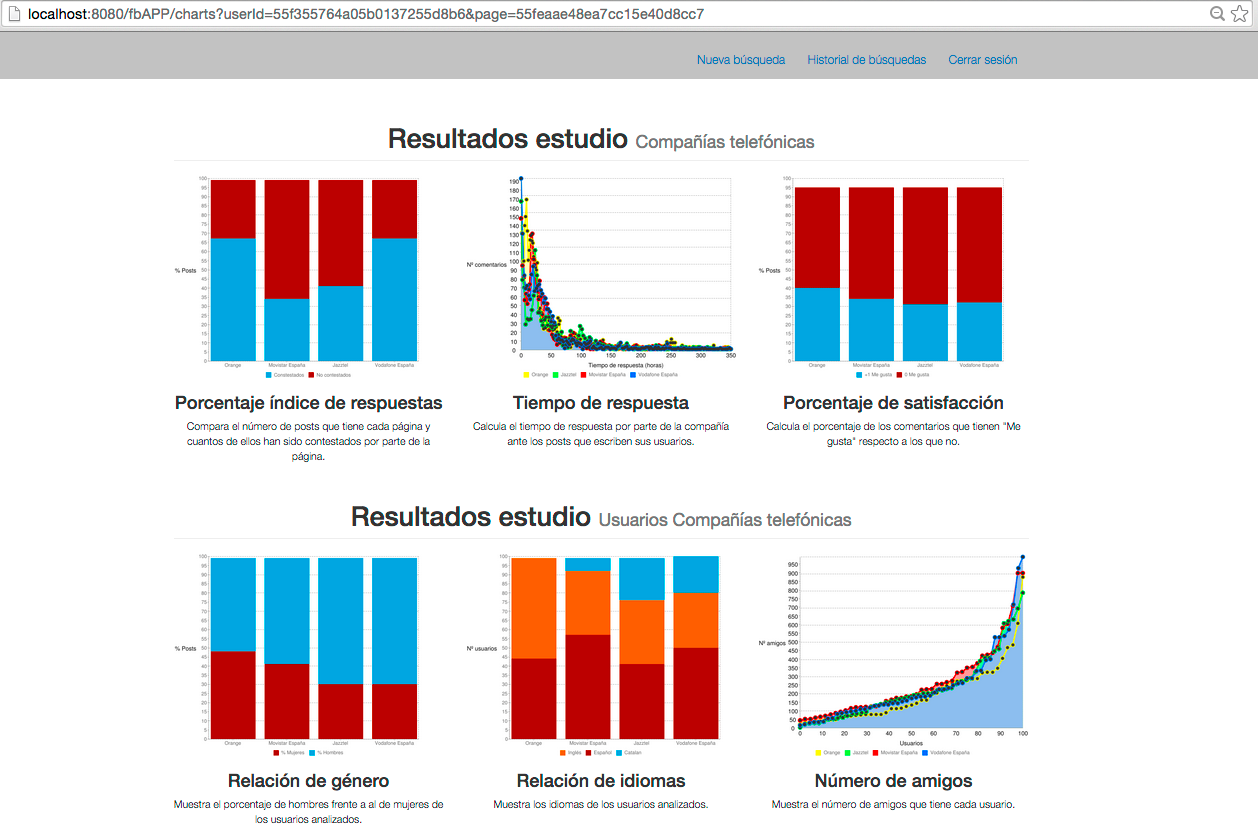
\includegraphics[width=5in]{figuras/ejemploAnalisis.png}
\caption{Captura de pantalla ejemplo análisis obtenido. Completo} \label{fig:exAnalisis}
\end{figure}
\end{itemize}
\chapter{Planificación del trabajo y presupuesto}
\section{Planificación del trabajo}
\subsection{Definición de tareas}
La elaboración del presente proyecto se ha dividido en tres fases, que se enumeran a continuaón:
\begin{itemize}
  \item \underline{FASE 1: Planificación}  \hfill  \\
  En todo proyecto antes de empezar a trabajar es necesario un estudio previo de los requisitos necesarios y de las posibles tecnologías para desarrollar el trabajo.
  \begin{itemize}
    \item \textit{Planteamiento del trabajo: }La primera tarea consistió en estudiar cuales eran los objetivos necesarios para la realización de este proyecto, su finalidad y una previa organización del mismo.
    \item \textit{Definición de requisitos: }Una vez examinados los objetivos indispensables, se realizó un listado de los requisitos tanto técnicos como materiales necesarios para llevar a cabo este proyecto.
    \item \textit{Estudio de sistemas de desarrollo: } El siguiente paso fue el análisis de las diferentes
alternativas para desarrollar este trabajo fin de grado, definiendo que lenguaje de programación utilizar, las tecnologías adecuadas, y la elección de la base de datos.
    \item \textit{Estudio de las tecnologías web: } Por último, se estudiaron las diferentes tecnologías web disponibles para desarrollar el portal web y las opciones que más convenían para este proyecto.
  \end{itemize}
  \item \underline{FASE 2: Desarrollo} \hfill \\
  
  2.1 BACKEND    
  \begin{itemize}
    \item \textit{Creación de las bases de datos:} Definido el proyecto, se empezó creando las bases de datos necesarias, una en MongoDB y otra en MySQL. Los requisitos de las bases de datos creadas se fueron incrementando en función de las necesidades de los programas que acceden a ellas.
    \item \textit{Creación script API de Facebook: } Después de crear un primer esquema de las bases de datos, el siguiente paso fue la realización del script que accedía a la API de Facebook. Hubo que analizar las diferentes posibilidades de acceder a la API de Facebook, los parámetros necesarios y la configuración adecuada.
    \item \textit{Creación del \textit{crawler} de Facebook: } Realizadas las primeras pruebas del script de la API de Facebook y teniendo los primeros datos para poder seguir avanzando con el proyecto, se procedió a desarrollar el \textit{crawler}, tarea que requería mayor tiempo de dedicación.
    \item \textit{Distribución del \textit{crawler} en distintas máquinas virtuales: }Desarrollado el \textit{crawler} casi por completo, se decidió montar una estructura para dividir el \textit{crawler} automáticamente en varias máquinas virtuales. Para esta parte se desarrolló un sistema de colas de mensajes con RabbitMQ que supuso también mucho tiempo de pruebas pero ayudó a definir mejor los requisitos del \textit{crawler}.
    \end{itemize}
    
    2.2 FRONTEND
    \begin{itemize}
    \item \textit{Implementación del diseño de la aplicación web: } En cuanto al \textit{frontend}, lo primero que se realizó fue una primera plantilla sencilla con un formulario que fuera capaz de introducir los datos indicados por un usuario en una base de datos. Una vez conseguido esto, se decidió el diseño de la web y se mejoraron
aspectos de estilo.
    \item \textit{Implementación del registro de usuarios: }Definidas las funcionalidades básicas de la aplicación web, se creó un sistema de registro/autenticación, para que sólo los usuarios registrados pudieran tener acceso a la aplicación.
    \item \textit{Implementación de las funcionalidades de la aplicación: } Una vez desarrolladas todas las partes necesarias para la creación de este proyecto, sólo faltaba unir los script creados en el \textit{backend} con la aplicación para que automáticamente parseará y obtuviera los datos de Facebook, los procesara y se los mostrara al usuario en la interfaz gráfica.
  \end{itemize}
  \item \underline{FASE 3: Evaluación y documentación} \hfill  \\
  El último bloque para finalizar el desarrollo de este trabajo fin de grado consistía en realizar pruebas de la aplicación y la redacción de la presente memoria, así como la preparación de la presentación del mismo.
    \begin{itemize}
    \item \textit{Pruebas aplicación:} Finalizado el sistema completo, se realizaron pruebas para comprobar el correcto funcionamiento y se llevaron a cabo un par de casos prácticos para explicar su funcionamiento en el presente documento.  
    \item \textit{Redacción de la memoria: } Redacción del presente documento.
    \item \textit{Preparación de la presentación.}
  \end{itemize}  
\end{itemize}

\subsection{Planificación: Diagrama de Gantt}
Una vez establecidas las tareas principales que definen el proyecto, se enmarcan dichas tareas en un intervalo temporal para establecer el tiempo estimado en la realización del mismo. Este periodo de tiempo se estima teniendo en cuenta el plazo máximo de entrega del proyecto, el 27 de Septiembre, y la disponibilidad del autor para la realización del trabajo. En este caso concreto, se ha requerido más tiempo ya que no se realizó a jornada completa.

En el diagrama de Gantt (\ref{tab:gantt}) se representan cada una de las fases definidas con el periodo de tiempo estimado. Se ha considerado el tiempo máximo disponible, 9 meses.
\begin{table}[H]
	\centering
	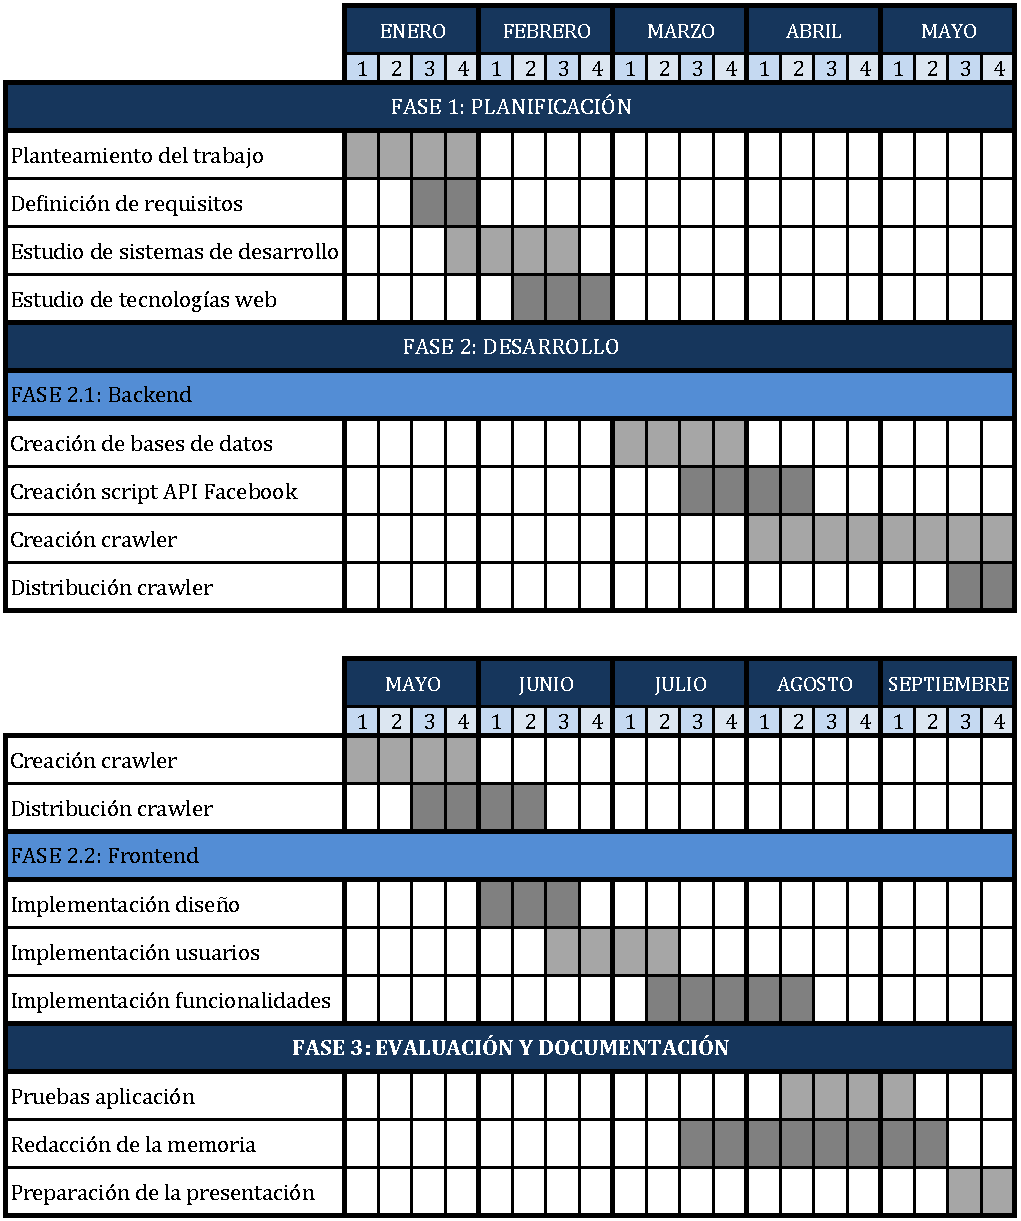
\includegraphics[width=6in]{PDF/DiagramadeGantt.pdf}
	\caption{Planificación del proyecto. Diagrama de Gantt}
	\label{tab:gantt}
\end{table}

\section{Presupuesto}
En el siguiente apartado se procede al calculo del presupuesto del proyecto realizado, detallando dos tipos de costes: costes materiales y costes de personal.
\subsection{Costes materiales}
En cuanto a costes materiales se han tenido en cuenta las siguientes variables:
\begin{itemize}
\item Portátil: Ordenador portátil de uso personal, marca Apple y modelo MacBook Air.
\item Software: El software utilizado para la realización del proyecto es de código abierto. Sólo se tiene en cuenta la utilización del paquete Microsoft Office para la realización de la documentación del proyecto. 
\item Servidor: Donde alojar OpenStack.
\item Material de oficina: Varios.
\item Alquiler de oficina: Estudio estimado de unos 20 metros cuadrados en Madrid. 
\item Gastos de luz y de internet.
\end{itemize}
\subsection{Costes de personal}
En cuanto a los costes de personal, se ha tenido en cuenta las horas dedicadas por parte del tutor, considerando el precio de la hora como Ingeniero Senior, y las horas dedicadas por parte de la autora del presente proyecto, contando las horas como Ingeniero Junior. 

Para estimar el precio de estas horas, según el Colegio de Ingenieros Técnicos de Telecomunicación (COITT) \cite{6}: \textit{"los honorarios son libres y responden al libre acuerdo entre el profesional y su cliente"}. 
\subsection{Costes totales}
En la siguiente tabla (\ref{tab:pres}) se calcula el presupuesto total del proyecto, teniendo en cuenta los costes comentados anteriormente. 
\begin{table}[H]
	\centering
	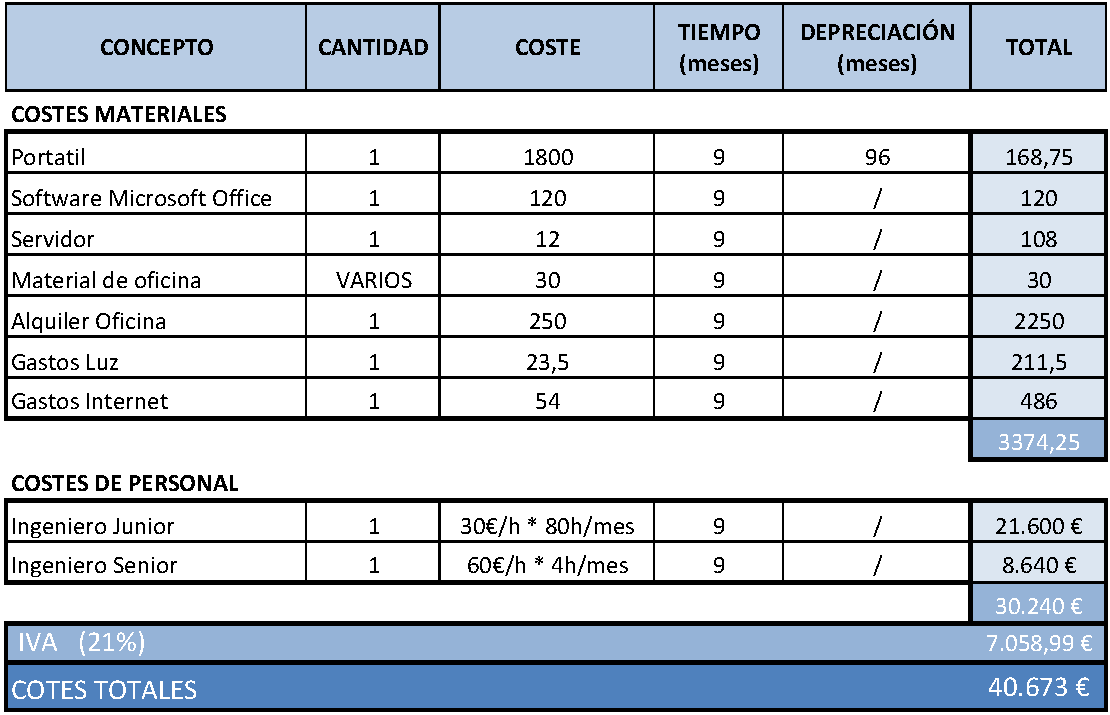
\includegraphics[width=5in]{PDF/Presupuesto.pdf}
	\caption{Presupuesto del proyecto}
	\label{tab:pres}
\end{table}
\chapter{Conclusiones}

Se presentan a continuación las conclusiones derivadas de la realización de este trabajo fin de grado. A su vez, se detallarán posibles mejoras aplicables para trabajos futuros.

\section{Conclusión}

En este trabajo fin de grado se ha desarrollado una aplicación web basada en el análisis estadístico de las páginas de Facebook. Esta aplicación ofrece al usuario la posibilidad de elegir las páginas que desea analizar y las características del estudio a realizar. Como se tratan de datos personales, el acceso a la aplicación está protegido de forma que sólo los usuarios registrados en la aplicación podrán tener acceso. Además de que sólo podrán ver sus datos y no los de ningún otro usuario. 

Gracias a la aplicación desarrollada, cualquier usuario puede conocer las características de una página de Facebook de manera automática, sin necesidad de recorrer cada una de las páginas e intuir en función de la actividad de la página cuáles son sus cualidades, o si hay algún factor que las haga distintivas respecto a otras. Se considera una aplicación pionera en ofrecer estos datos a usuarios externos, ya que, actualmente, no existe ninguna aplicación conocida que sea capaz de realizar esto con los datos relacionados de Facebook. 

Se trata de una aplicación de gran utilidad para las empresas, si lo que desean es ampliar su mercado mediante las redes sociales, distinguiéndose del resto.
Los datos proporcionados por la aplicación, pueden servir para aplicar tareas de marketing a raíz dichos datos. Mediante dichos datos se puede conocer cómo actúan sus mayores competidores y mejorar los aspectos que consideren oportunos.

Para la realización de las funcionalidades de esta aplicación se ha tenido que desarrollar un programa capaz de recoger y almacenar todos los datos necesarios de las páginas de Facebook a través de su API, además de la realización de un \textit{crawler} capaz de recoger todos los datos de los usuarios de Facebook.

Destacar también un mayor grado de dificultad de este trabajo manejando dos tipos de bases de datos distintos, lo que ha supuesto un reto más. Además de tener que aplicarse diferentes tecnologías para su realización.

Concluyendo, a pesar de la complejidad de alguna de las tareas realizadas, los objetivos del presente proyecto han sido concluidos por completo. Además el trabajo realizado ha servido de gran aprendizaje para la autora del mismo. Por lo tanto se puede concluir el trabajo con una valoración muy positiva del mismo.

\section{Desarrollos futuros}
Para concluir con la documentación de este trabajo fin de grado se proponen varias mejoras posibles para un trabajo futuro.
\begin{itemize}
\item \textbf{Mejorar la accesibilidad de los usuarios:} Integrar la aplicación en diferentes plataformas como \textit{Android} e \textit{iOS}, para permitir su accesibilidad desde dispositivos móviles.
\item \textbf{Añadir más funcionalidades a la aplicación:} Añadir más gráficas al estudio, para obtener un análisis más completo. También se puede mejorar el formulario de búsqueda ofreciendo a los usuarios el resultado de las búsquedas de páginas en Facebook, eliminando el paso de comprobación del nombre y de la existencia de la sección \textit{Post To Page}. 
\item \textbf{Definir mejor los resultados realizando análisis de sentimiento:} Incluir análisis de texto para identificar y extraer información subjetiva de los comentarios de los usuarios, este procesado de los datos intenta determinar la actitud de un usuario ante un suceso. Con esta mejora se podrían calificar los comentarios como positivos o negativos, pudiendo deducir si son quejas o expresan gratitud.  
\item \textbf{Mejorar la concurrencia del sistema:} Dividir en hilos las consultas a la API de Facebook, de forma que se reduzca el tiempo de espera del usuario.
\end{itemize}

%%%%%%%%%%%%%%%%%%%%%%%%%%%%%%%%%%%%%%%%%%%%%%%%%%%%%%%%%%%%%%%%%%%%%%
%                           APÉNDICES
%%%%%%%%%%%%%%%%%%%%%%%%%%%%%%%%%%%%%%%%%%%%%%%%%%%%%%%%%%%%%%%%%%%%%%
%\appendix
%\input{./Apendices/ApendiceA}
%\input{./Apendices/ApendiceB}
%\input{./Apendices/ApendiceB}
%\input{./Apendices/ApendiceC}
%\backmatter

%%%%%%%%%%%%%%%%%%%%%%%%%%%%%%%%%%%%%%%%%%%%%%%%%%%%%%%%%%%%%%%%%%%%%%
%                       BIBLIOGRAFÍA
%%%%%%%%%%%%%%%%%%%%%%%%%%%%%%%%%%%%%%%%%%%%%%%%%%%%%%%%%%%%%%%%%%%%%%


% Para compilar: bibtex MemoriaPFC
% Luego darle a componer
%Para poner la bibliografía. El ieeetr es el estilo y lo de abajo son los
%ficheros .bib que tienes que cargar. Los debes crear tu o coger algunos ya
%creados con tus referencias.
\begin{flushleft}
\bibliographystyle{plain}
\bibliography{bibliografia}

\nocite{*} %%% OJO: descomentado incluye todas las referencias, hayan sido citadas o no.

\end{flushleft}

%%%%%%%%%%%%%%%%%%%%%%%%%%%%%%%%%%%%%%%%%%%%%%%%%%%%%%%%%%%%%%%%%%%%%%
%                       FIN DEL DOCUMENTO
%%%%%%%%%%%%%%%%%%%%%%%%%%%%%%%%%%%%%%%%%%%%%%%%%%%%%%%%%%%%%%%%%%%%
\end{document}